% Options for packages loaded elsewhere
\PassOptionsToPackage{unicode}{hyperref}
\PassOptionsToPackage{hyphens}{url}
\PassOptionsToPackage{dvipsnames,svgnames,x11names}{xcolor}
\documentclass[
  spanish,
  10pt,
  a4paper,
]{article}
\usepackage{xcolor}
\usepackage[top=22mm,bottom=22mm,left=22mm,right=22mm]{geometry}
\usepackage{amsmath,amssymb}
\setcounter{secnumdepth}{-\maxdimen} % remove section numbering
\usepackage{iftex}
\ifPDFTeX
  \usepackage[T1]{fontenc}
  \usepackage[utf8]{inputenc}
  \usepackage{textcomp} % provide euro and other symbols
\else % if luatex or xetex
  \usepackage{unicode-math} % this also loads fontspec
  \defaultfontfeatures{Scale=MatchLowercase}
  \defaultfontfeatures[\rmfamily]{Ligatures=TeX,Scale=1}
\fi
\usepackage{lmodern}
\ifPDFTeX\else
  % xetex/luatex font selection
\fi
% Use upquote if available, for straight quotes in verbatim environments
\IfFileExists{upquote.sty}{\usepackage{upquote}}{}
\IfFileExists{microtype.sty}{% use microtype if available
  \usepackage[]{microtype}
  \UseMicrotypeSet[protrusion]{basicmath} % disable protrusion for tt fonts
}{}
\usepackage{setspace}
\makeatletter
\@ifundefined{KOMAClassName}{% if non-KOMA class
  \IfFileExists{parskip.sty}{%
    \usepackage{parskip}
  }{% else
    \setlength{\parindent}{0pt}
    \setlength{\parskip}{6pt plus 2pt minus 1pt}}
}{% if KOMA class
  \KOMAoptions{parskip=half}}
\makeatother
\usepackage{longtable,booktabs,array}
\newcounter{none} % for unnumbered tables
\usepackage{calc} % for calculating minipage widths
% Correct order of tables after \paragraph or \subparagraph
\usepackage{etoolbox}
\makeatletter
\patchcmd\longtable{\par}{\if@noskipsec\mbox{}\fi\par}{}{}
\makeatother
% Allow footnotes in longtable head/foot
\IfFileExists{footnotehyper.sty}{\usepackage{footnotehyper}}{\usepackage{footnote}}
\makesavenoteenv{longtable}
\usepackage{graphicx}
\makeatletter
\newsavebox\pandoc@box
\newcommand*\pandocbounded[1]{% scales image to fit in text height/width
  \sbox\pandoc@box{#1}%
  \Gscale@div\@tempa{\textheight}{\dimexpr\ht\pandoc@box+\dp\pandoc@box\relax}%
  \Gscale@div\@tempb{\linewidth}{\wd\pandoc@box}%
  \ifdim\@tempb\p@<\@tempa\p@\let\@tempa\@tempb\fi% select the smaller of both
  \ifdim\@tempa\p@<\p@\scalebox{\@tempa}{\usebox\pandoc@box}%
  \else\usebox{\pandoc@box}%
  \fi%
}
% Set default figure placement to htbp
\def\fps@figure{htbp}
\makeatother
\ifLuaTeX
\usepackage[bidi=basic,shorthands=off]{babel}
\else
\usepackage[bidi=default,shorthands=off]{babel}
\fi
\ifLuaTeX
  \usepackage{selnolig} % disable illegal ligatures
\fi
\setlength{\emergencystretch}{3em} % prevent overfull lines
\providecommand{\tightlist}{%
  \setlength{\itemsep}{0pt}\setlength{\parskip}{0pt}}

\usepackage{amsmath,amssymb,mathtools}
\usepackage{microtype}
\usepackage{fancyhdr}
\usepackage{needspace}
\usepackage{etoolbox}
\usepackage{float}
\usepackage{caption}
\captionsetup{font=small,labelformat=empty,skip=7pt}
\floatplacement{figure}{H}
\definecolor{DocBlue}{HTML}{173F57}
\definecolor{DocGray}{HTML}{52616C}
\pagestyle{fancy}
\fancyhf{}
\fancyhead[L]{\small\sffamily\color{DocGray} pySNSPD | Desarrollo del modelo}
\fancyhead[R]{\small\sffamily\color{DocGray} Revisión 0.4}
\fancyfoot[L]{\small\sffamily\color{DocGray} 9 de septiembre de 2026}
\fancyfoot[R]{\small\sffamily\thepage}
\setlength{\headheight}{15pt}
\setlength{\emergencystretch}{2em}
\setlength{\parskip}{5pt plus 1pt}
\setlength{\parindent}{0pt}
\widowpenalty=10000
\clubpenalty=10000
\displaywidowpenalty=10000
\predisplaypenalty=10000
\renewcommand{\arraystretch}{1.16}
\AtBeginEnvironment{longtable}{\small}
\pretocmd{\section}{\Needspace{6\baselineskip}}{}{}
\pretocmd{\subsection}{\Needspace{5\baselineskip}}{}{}
\AtBeginDocument{\hypersetup{colorlinks=true,linkcolor=DocBlue,urlcolor=DocBlue}}
\allowdisplaybreaks[1]
\usepackage{bookmark}
\IfFileExists{xurl.sty}{\usepackage{xurl}}{} % add URL line breaks if available
\urlstyle{same}
\hypersetup{
  pdftitle={B. Cinética{,} energía y temperaturas},
  pdfauthor={Desarrollo del modelo pySNSPD},
  pdflang={es},
  colorlinks=true,
  linkcolor={Maroon},
  filecolor={Maroon},
  citecolor={Blue},
  urlcolor={Blue},
  pdfcreator={LaTeX via pandoc}}

\title{B. Cinética, energía y temperaturas}
\usepackage{etoolbox}
\makeatletter
\providecommand{\subtitle}[1]{% add subtitle to \maketitle
  \apptocmd{\@title}{\par {\large #1 \par}}{}{}
}
\makeatother
\subtitle{Actualización física y pedagógica de pySNSPD · Documento
técnico 2 de 5}
\author{Desarrollo del modelo pySNSPD}
\date{9 de septiembre de 2026 · Revisión 0.4}

\begin{document}
\maketitle

{
\setcounter{tocdepth}{2}
\tableofcontents
}
\setstretch{1.07}
\newpage

\section{B.0. Modelo cinético adoptado y alcance de esta
revisión}\label{b.0.-modelo-cinuxe9tico-adoptado-y-alcance-de-esta-revisiuxf3n}

\textbf{Decisión.} Se conservan las ocupaciones electrónicas y fonónicas
completas durante todo el tiempo de cálculo. La temperatura equivalente
expresa su energía y permite evaluar el cierre disipativo; no sustituye
esas poblaciones. Se retiran el cambio automático a dos temperaturas, la
reducción por momentos y las bandas fonónicas. La figura B.2 muestra por
qué la energía sola no determina la fuerza y cuánto depende su
relajación de una tasa cinética aún no identificada para la película.

{\def\LTcaptype{none} % do not increment counter
\begin{longtable}[]{@{}
  >{\raggedright\arraybackslash}p{(\linewidth - 4\tabcolsep) * \real{0.3333}}
  >{\raggedright\arraybackslash}p{(\linewidth - 4\tabcolsep) * \real{0.3333}}
  >{\raggedright\arraybackslash}p{(\linewidth - 4\tabcolsep) * \real{0.3333}}@{}}
\toprule\noalign{}
\begin{minipage}[b]{\linewidth}\raggedright
Parte del modelo 0.4
\end{minipage} & \begin{minipage}[b]{\linewidth}\raggedright
Elección adoptada
\end{minipage} & \begin{minipage}[b]{\linewidth}\raggedright
Diagnóstico que la respalda o limita
\end{minipage} \\
\midrule\noalign{}
\endhead
\bottomrule\noalign{}
\endlastfoot
Poblaciones & \(f(E,\mathbf r,t)\) y \(n(\Omega,\mathbf r,t)\)
espectrales en todo el dominio y tiempo & Igual energía produce fuerzas
diferentes; B.5 y figura B.2 \\
Colisiones & Reacciones electrón--fonón apareadas y relajación
electrónica conservativa & Trayectorias nuevas, balance detallado y
refinamiento; B.10 \\
Transporte & Difusión electrónica longitudinal; escape fonónico local al
sustrato & Prueba de dos celdas; transporte lateral de fonones omitido
explícitamente \\
Calor & Fuente espectral fenomenológica B.41, definida también desde el
vacío & B.9: momento energético exacto, límite térmico y trayectoria
desde \(p=0\) \\
Material & DOS de modos por volumen y energía, positiva y con
normalización documentada & La tabla NbN disponible no supera la
admisión; B.7.2 \\
Condensado & Espectro local del candidato regular de C, con
\(\mathbf q=\mathbf q_\delta\) & La corriente física se obtiene variando
la energía completa de C \\
\end{longtable}
}

Éste es un \textbf{candidato continuo cerrado para ensayos}, con
parámetros y requisitos de entrada explícitos. Cerrar sus ecuaciones no
equivale a validar la descripción microscópica de la disipación, el
núcleo de un vórtice o las tasas absolutas de NbN. No se modifica
producción en esta revisión.

A entrega el catálogo estático y B.11 deriva su extensión adiabática. En
las fórmulas locales de B, \(\mathbf q\) es el argumento formal del
catálogo; el modelo integrado lo evalúa siempre en
\(\mathbf q_\delta=\operatorname{Im}[\Delta^*\mathcal D\Delta]/(|\Delta|^2+\delta^2)\),
con \(\mathcal D=\nabla-2ie\mathbf A/\hbar\) y el valor finito de
\(\delta\) fijado en C. Se usa ese mismo espectro en las energías,
fuerzas, colisiones y transporte. \(\dot{\mathbf q}_\delta\) incluye la
variación de \(\Delta\) y de sus gradientes; no es un grado de libertad
independiente. La fuerza \(\boldsymbol\Pi\) de B.50 alimenta la
variación de C: por sí sola no es la corriente física regularizada.

\section{B.1. Variables y tres significados diferentes de
temperatura}\label{b.1.-variables-y-tres-significados-diferentes-de-temperatura}

\textbf{La etiqueta FD no designa la misma magnitud en A y B.} Aquí

\[
f_{\rm FD}(E,T)=\frac{1}{\exp[E/(k_BT)]+1}
\]

es la ocupación de un estado de excitación: un número adimensional entre
cero y uno. En A, \(f_e^{\rm FD}(T,|\Delta|,q)\) es una \textbf{densidad
de energía libre electrónica}, con unidades J/m\(^3\), evaluada para
ocupaciones Fermi--Dirac. Comparten la etiqueta porque una usa la
población térmica que define a la otra; no se igualan ni se sustituyen
entre sí.

{\def\LTcaptype{none} % do not increment counter
\begin{longtable}[]{@{}
  >{\raggedright\arraybackslash}p{(\linewidth - 4\tabcolsep) * \real{0.3333}}
  >{\raggedright\arraybackslash}p{(\linewidth - 4\tabcolsep) * \real{0.3333}}
  >{\raggedright\arraybackslash}p{(\linewidth - 4\tabcolsep) * \real{0.3333}}@{}}
\toprule\noalign{}
\begin{minipage}[b]{\linewidth}\raggedright
Símbolo
\end{minipage} & \begin{minipage}[b]{\linewidth}\raggedright
Objeto
\end{minipage} & \begin{minipage}[b]{\linewidth}\raggedright
Unidades y operación típica
\end{minipage} \\
\midrule\noalign{}
\endhead
\bottomrule\noalign{}
\endlastfoot
\(f(E)\), \(f_{\rm FD}(E,T)\) & Ocupación de un estado & Adimensional;
entra en \(f(1-f')\) \\
\(f_e^{\rm FD}\) & Densidad de energía libre & J/m\(^3\); sus derivadas
dan entropía y fuerzas \\
\(u_e\), \(u_{\rm qp}\) & Densidades de energía interna y de
excitaciones & J/m\(^3\); entran en balances \\
\end{longtable}
}

El puente es sumar energías de estados \textbf{pesadas por sus
ocupaciones}, como en B.19, y después incluir la entropía, como en B.23
y B.46--B.48. Por ejemplo, en B.40 se abrevia \(f=f_e^{\rm FD}\) sólo
dentro del balance térmico; en las colisiones B.3--B.6, \(f\) siempre
significa ocupación. Las clases de cálculo funcional de E practican la
diferencia entre función y funcional; las clases sobre modos, DOS y DFPT
conectan el conteo de modos con \(g_{\rm ph}\) y \(\alpha^2F\).

Los campos son \(\Delta=|\Delta| e^{i\theta}\), \(\mathbf q\), las
ocupaciones electrónicas \(f(E,\mathbf r,t)\) y fonónicas
\(n(\Omega,\mathbf r,t)\). Se presupone simetría electrón--hueco; el
desequilibrio de carga espectral independiente no está resuelto en esta
versión. Las funciones de Usadel son \(\rho=N_1\), \(N_2\) y \(R_2\).

Conviene separar tres situaciones. Si \(f=f_{\rm FD}(E,T_e)\), \(T_e\)
es una temperatura de cuasiequilibrio. Si \(f\) no es Fermi--Dirac,
\(T_E\) es la temperatura de una distribución térmica con la misma
energía: una coordenada útil, pero no una descripción completa. Si
existe un pequeño subsistema térmico más una cola no térmica, la
temperatura de ese subsistema no coincide necesariamente con \(T_E\) del
conjunto. El modelo 0.4 no introduce ese tercer reparto.

Una analogía útil es una cuenta bancaria: el saldo total no indica si
está repartido en muchas monedas pequeñas o en pocos billetes grandes.
\(u_{\rm qp}\) es el saldo; \(f(E)\) describe el reparto. Las colisiones
y la fuerza sobre el condensado responden también a ese reparto. La
figura B.2 lo cuantifica sin simular una cascada.

{\def\LTcaptype{none} % do not increment counter
\begin{longtable}[]{@{}
  >{\raggedright\arraybackslash}p{(\linewidth - 4\tabcolsep) * \real{0.3333}}
  >{\raggedright\arraybackslash}p{(\linewidth - 4\tabcolsep) * \real{0.3333}}
  >{\raggedright\arraybackslash}p{(\linewidth - 4\tabcolsep) * \real{0.3333}}@{}}
\toprule\noalign{}
\begin{minipage}[b]{\linewidth}\raggedright
Variable
\end{minipage} & \begin{minipage}[b]{\linewidth}\raggedright
Información que conserva
\end{minipage} & \begin{minipage}[b]{\linewidth}\raggedright
Qué no determina por sí sola
\end{minipage} \\
\midrule\noalign{}
\endhead
\bottomrule\noalign{}
\endlastfoot
\(f(E),n(\Omega)\) & Ocupación de cada intervalo espectral & Su
evolución exige transporte y colisiones \\
\(u_{\rm qp},u_{\rm ph}\) & Energía de cada sector & Forma de la
distribución \\
\(T_E,T_{{\rm ph},E}\) & La misma energía, escrita en una escala térmica
& Fuerza, corriente o tasas fuera de equilibrio \\
\(T_e,T_{\rm ph}\) & Distribuciones térmicas completas, si el cierre es
válido & Correcciones no térmicas descartadas \\
\end{longtable}
}

La biyección de B.20 será entre \textbf{energía y temperatura
equivalente a espectro fijo}, no entre una distribución arbitraria y una
temperatura.

\section{B.2. Coherencia superconductora y espacio de fases
correcto}\label{b.2.-coherencia-superconductora-y-espacio-de-fases-correcto}

\textbf{Propósito.} Usar las mismas funciones espectrales para decidir
cuántos estados existen y con qué peso intervienen en cada reacción. Los
factores de coherencia expresan que una cuasipartícula superconductora
mezcla componentes de electrón y de hueco; esa mezcla afecta de forma
distinta a la dispersión y a la recombinación.

La memoria combina DOS de Usadel con factores BCS
\(1\mp |\Delta|^2/(EE')\) y límites de integración asociados al gap BCS.
Su anexo A reconoce esta aproximación. Los núcleos propuestos utilizan
el espectro normal y el anómalo del mismo problema {[}M, V{]}:

\[
\begin{gathered}
\mathcal C_S(E,E')=N_1(E)N_1(E')-R_2(E)R_2(E'),\\
\mathcal C_R(E,E')=N_1(E)N_1(E')+R_2(E)R_2(E').
\end{gathered} \tag{B.1}
\]

En el límite BCS sin corriente se recupera

\[
\begin{gathered}
R_2(E)=\rho(E)\frac{|\Delta|}{E},\\
\mathcal C_{S/R}=\rho(E)\rho(E')\left(1\mp\frac{|\Delta|^2}{EE'}\right).
\end{gathered} \tag{B.2}
\]

La nueva expresión no añade un mecanismo: deja de aplicar fuera de su
límite una simplificación del mismo mecanismo. La no negatividad de los
núcleos y la rama física deben verificarse. No se obtiene una teoría
fiable recortando a cero valores negativos producidos por ramas
espectrales incompatibles.

Se integrará sobre \(E>0\) y \(\Omega>0\). El soporte espectral
determina los umbrales. Bajo depairing, el borde de DOS \(E_g\) no es
\(|\Delta|\); por ello no se conserva un corte artificial en
\(|\Delta|\) o \(2|\Delta|\). El ensanchamiento \(\eta\) se trata como
regulador o parámetro físico identificado, no como una tasa inelástica
universal.

\section{B.3. Reacciones elementales y balance
energético}\label{b.3.-reacciones-elementales-y-balance-energuxe9tico}

\textbf{Propósito.} Construir ambos balances a partir de la misma lista
de reacciones. Así se evita que electrones y fonones cuenten cantidades
ligeramente diferentes de la misma transferencia.

\begin{figure}
\centering

\includegraphics[width=0.96\linewidth,height=\textheight,keepaspectratio,alt={Figura B.1. Recurso pedagógico: cada reacción retira de los electrones exactamente la energía del fonón creado. Las energías son ejemplos arbitrarios; el espectro se mantiene fijo durante la colisión. La recuperación posterior de la amplitud se contabiliza aparte en B.9 y C.}]{../figuras/B_01_reacciones_balance.png}
\caption{Figura B.1. Recurso pedagógico: cada reacción retira de los
electrones exactamente la energía del fonón creado. Las energías son
ejemplos arbitrarios; el espectro se mantiene fijo durante la colisión.
La recuperación posterior de la amplitud se contabiliza aparte en B.9 y
C.}
\end{figure}

\subsection{B.3.1. Factores de
ocupación}\label{b.3.1.-factores-de-ocupaciuxf3n}

Para la emisión neta de un fonón de energía \(\Omega\) por una
cuasipartícula que pasa de \(E+\Omega\) a \(E\),

\[
\mathcal B_S=f(E+\Omega)[1-f(E)](n+1)
-f(E)[1-f(E+\Omega)]n. \tag{B.3}
\]

Para recombinación neta de dos cuasipartículas de energías \(E\) y
\(\Omega-E\),

\[
\mathcal B_R=f(E)f(\Omega-E)(n+1)
-[1-f(E)][1-f(\Omega-E)]n. \tag{B.4}
\]

El signo positivo representa creación neta de fonones; un signo negativo
representa absorción o ruptura de pares.

Cada producto se lee de izquierda a derecha: ocupación inicial,
disponibilidad del estado final y ocupación fonónica. \(1-f\) impide
llegar a un estado electrónico ocupado; \(n+1\) incorpora emisión
espontánea y estimulada. La resta compara el proceso directo con el
inverso. No es necesario asignarles un signo de calentamiento por
separado. Se definen las densidades de reacción, con \(N_0\) por espín,

\[
\begin{gathered}
\mathcal R_S(E,\Omega)=\frac{8\pi N_0}{\hbar}
\alpha^2F(\Omega)\mathcal C_S(E,E+\Omega)\mathcal B_S,\\
0<E<\infty,
\end{gathered} \tag{B.5}
\]

\[
\begin{gathered}
\mathcal R_R(E,\Omega)=\frac{4\pi N_0}{\hbar}
\alpha^2F(\Omega)\mathcal C_R(E,\Omega-E)\mathcal B_R,\\
0<E<\Omega.
\end{gathered} \tag{B.6}
\]

El factor relativo \(1/2\) evita contar dos veces el mismo par al
recorrer \(E\) y \(\Omega-E\). En B.5--B.6, \(\alpha^2F\) tiene la
convención adimensional del eje de energía utilizada en A. Una
implementación que use otra convención debe transformar los prefactores,
no copiar ambas simultáneamente.

\subsection{B.3.2. Ecuación débil para cualquier momento
electrónico}\label{b.3.2.-ecuaciuxf3n-duxe9bil-para-cualquier-momento-electruxf3nico}

Para un peso \(b(E)\), sea

\[
m_b=4N_0\int_0^\infty b(E)\rho(E)f(E)\,dE.
\]

Durante las colisiones, el espectro se mantiene fijo. El cambio debido a
B.5--B.6 es el número neto de reacciones multiplicado por el cambio de
la cantidad observada. En dispersión ese cambio es \(b(E)-b(E+\Omega)\);
en recombinación se pierden ambos pesos. Por tanto,

\[
\begin{aligned}
\left.\dot m_b\right|_{e\text{-ph}}={}&
\int_0^\infty d\Omega\int_0^\infty dE\,
[b(E)-b(E+\Omega)]\mathcal R_S\\
&-\int_0^\infty d\Omega\int_0^\Omega dE\,
[b(E)+b(\Omega-E)]\mathcal R_R.
\end{aligned} \tag{B.7}
\]

Para \(b=1\), la dispersión conserva el número de cuasipartículas y cada
recombinación lo reduce en dos. Para \(b=E\), el corchete de dispersión
vale \(-\Omega\), mientras el de recombinación vale \(\Omega\). Por
tanto,

\[
\left.\dot u_e\right|_{e\text{-ph}}=-P_{e\text{-ph}}, \tag{B.8}
\]

\[
P_{e\text{-ph}}=\int_0^\infty\Omega\left[
\int_0^\infty\mathcal R_S\,dE+
\int_0^\Omega\mathcal R_R\,dE\right]d\Omega. \tag{B.9}
\]

No se decide el signo de la fila fonónica por conveniencia: cada
reacción añade o retira exactamente el fonón que aparece en B.9.

\subsection{B.3.3. Ecuación de
fonones}\label{b.3.3.-ecuaciuxf3n-de-fonones}

La ecuación sigue la población de modos, tanto si forman una
distribución térmica como si constituyen una \textbf{burbuja fonónica}:
un exceso localizado de fonones de alta energía. ``Burbuja'' describe
dónde está inicialmente la energía y en qué sector, sin implicar una
cavidad material ni una temperatura única.

Vodolazov compara condiciones iniciales electrónica, fonónica y térmica
a igual energía, y encuentra que el reparto y la termalización dependen
de la razón de capacidades electrón/fonón. Su burbuja fonónica es una
condición de prueba; no identifica toda absorción óptica con un
calentamiento Bose instantáneo. Esto respalda separar la energía
inyectada de la forma inicial de las ocupaciones {[}V, §III, ecuaciones
(16)--(22), pp.~4--6 del preprint{]}.

La tesis de Allmaras sigue el paso de excitaciones electrón--hueco a
fonones de primera generación y su posterior reabsorción. Sus cálculos
muestran por qué, después de una etapa temprana no resuelta, una
población fonónica puede servir como condición de entrada; también
muestran que forzar electrones térmicos puede transferirles energía
demasiado rápido. La ``burbuja modificada'' ralentiza ese intercambio
como corrección efectiva, no como una nueva ley microscópica {[}A,
§§2.3.1--2.3.2 y 2.4.6{]}. En la ecuación B.10 se conserva el
intercambio espectral para poder contrastar ese cierre; la sección B.8
especifica el instante y la energía que entrega la etapa omitida.

Con \(g_{\rm ph}(\Omega)\) como DOS fonónica por volumen y por energía,
fijada en B.7.2,

\[
g_{\rm ph}(\Omega)\dot n(\Omega)=
\int_0^\infty\mathcal R_S\,dE+
\int_0^\Omega\mathcal R_R\,dE
-\frac{g_{\rm ph}(\Omega)}{\tau_{\rm esc}}[n-n_b]
+S_{\gamma,\rm ph}(\Omega). \tag{B.10}
\]

Su momento energético da

\[
\begin{gathered}
u_{\rm ph}=\int_0^\infty g_{\rm ph}(\Omega)\Omega n(\Omega)\,d\Omega,\\
\dot u_{\rm ph}=P_{e\text{-ph}}-P_{\rm esc}+S_{\gamma,\rm ph}^{(E)},
\end{gathered} \tag{B.11}
\]

\[
P_{\rm esc}=\int_0^\infty
\frac{g_{\rm ph}(\Omega)\Omega[n-n_b]}{\tau_{\rm esc}}\,d\Omega. \tag{B.12}
\]

Sin escape ni fuentes, B.8 y B.11 cancelan exactamente el intercambio.
Esta cancelación es independiente de si \(f\) o \(n\) son térmicas. Debe
preservarse al discretizar el espectro.

\textbf{Prueba nueva de trayectoria.} B.10 integra ambas poblaciones en
dos celdas con difusión electrónica y escape. En la malla más fina, la
suma de energía electrónica, fonónica y escape acumulado conserva su
valor inicial con residuo relativo \(2.02\times10^{-16}\). Esta prueba
añade evolución temporal a la contabilidad de eventos de 0.3; usa un
espectro normal sintético, no tasas materiales de NbN.

Se adopta un único tiempo de escape efectivo, constante en energía:
\(\tau_{\rm esc}=15\) ps en el escenario de configuración existente. Es
una entrada de interfaz heredada, no un resultado de la auditoría 0.4.
En esta aproximación no hay difusión lateral de fonones ni
redistribución fonón--fonón. Esa elección permite evaluar el candidato
local con un balance identificable; su validez exige comprobar que el
recorrido lateral relevante y la redistribución omitida no cambian el
reparto antes de reabsorber o escapar. La tabla isotrópica \(F\) no
contiene velocidades, ángulos ni libres recorridos y no puede resolver
esa comprobación por sí sola.

\section{B.4. Transporte, evolución del espectro y colisiones
electrón--electrón}\label{b.4.-transporte-evoluciuxf3n-del-espectro-y-colisiones-electruxf3nelectruxf3n}

\textbf{Propósito.} Separar tres cambios que pueden ocurrir
simultáneamente: una ocupación se desplaza en el espacio, una colisión
redistribuye población y el condensado mueve la energía de los estados.
Sólo los dos primeros cambian directamente la población del estado que
se sigue.

\subsection{B.4.1. Difusión electrónica
espectral}\label{b.4.1.-difusiuxf3n-electruxf3nica-espectral}

En el cierre longitudinal de energía de Vodolazov,

\[
\begin{gathered}
\mathcal D_L(E)=N_1^2(E)-R_2^2(E),\\
\boldsymbol\Phi_f(E)=-4N_0D\mathcal D_L(E)\nabla_E f(E).
\end{gathered} \tag{B.13}
\]

La notación \(\nabla_E\) indica una derivada espacial a energía
espectral fija. El flujo de energía es

\[
\mathbf Q_e=\int_0^\infty E\boldsymbol\Phi_f(E)\,dE.
\tag{B.14}
\]

La divergencia del flujo se añade a la ecuación espectral antes de
reducirla. Cuando el peso \(b\) depende de los campos locales, el
momento de transporte es

\[
-\int b\nabla\cdot\boldsymbol\Phi_f\,dE
=-\nabla\cdot\int b\boldsymbol\Phi_f\,dE
+\int(\nabla_Eb)\cdot\boldsymbol\Phi_f\,dE. \tag{B.15}
\]

Ignorar el segundo término para los momentos de fuerza no es una
reducción exacta. B.13 es el sector de energía de la aproximación
adoptada; no sustituye todas las ecuaciones de desequilibrio de carga y
respuesta electromagnética de Keldysh.

\subsection{B.4.2. Derivada temporal a estados
fijos}\label{b.4.2.-derivada-temporal-a-estados-fijos}

Piénsese en pasajeros sobre los peldaños de una escalera mecánica:
cambiar de peldaño y mover la escalera son operaciones diferentes. \(x\)
etiqueta el estado; \(E(x,t)\) es su energía instantánea. En ausencia de
colisiones un estado puede conservar su ocupación aunque cambie la
función dibujada frente al eje \(E\). La regla de la cadena distingue
ambas operaciones.

Con la coordenada de estados \(x\) de B.43 y sus derivadas B.45,

\[
\begin{gathered}
\left.\dot p\right|_x=
\left.\partial_tf\right|_E+\dot E|_x\,\partial_Ef,\\
\dot E|_x=\frac{R_2}{\rho}\partial_t|\Delta|
-\hbar D\frac{N_2R_2}{\rho}\mathbf q\cdot\dot{\mathbf q}.
\end{gathered} \tag{B.16}
\]

El primer término proporcional a \(\partial_t|\Delta|\) es la estructura
que aparece en la ecuación cinética de Vodolazov. La variación del
espectro no puede omitirse y después compensarse únicamente reajustando
\(C_e\). La misma derivada produce el almacenamiento en amplitud y
superflujo al tomar el momento energético.

Las ecuaciones de ocupación quedan definidas por B.7 para las
reacciones, B.13--B.16 para el transporte y la deriva espectral, y los
operadores adicionales explícitos de electrones y fuentes. Es una
formulación débil equivalente a evolucionar el espectro cuando se
conserva un conjunto completo de pesos. Un número finito de pesos
introduce un cierre nuevo.

\subsection{B.4.3. Relajación electrónica efectiva
conservativa}\label{b.4.3.-relajaciuxf3n-electruxf3nica-efectiva-conservativa}

Se adopta un único operador de relajación hacia Fermi--Dirac, de tipo
BGK:

\[
\left.\dot p\right|_{ee}
=\frac{f_{\rm FD}(E(x),T_E)-p(x)}{\tau_{\rm kin}}.
\tag{B.17}
\]

\(\tau_{\rm kin}>0\) es constante sobre la energía en una celda e
instante. Es un tiempo cinético de entrada; no se identifica
automáticamente con el \(\tau_{ee}\) que modifica la movilidad KWT de C.
En particular, los \(0.5\) ps a \(T_c\) de la configuración no
constituyen una calibración de B.17. Se requiere identificar
\(\tau_{\rm kin}\) mediante una relajación espectral o datos cinéticos
de la película antes de predecir tiempos absolutos.

\(T_E\) conserva la energía por B.20, de modo que

\[
4N_0\int_0^\infty E\left.\dot p\right|_{ee}dx=0.
\tag{B.18}
\]

Para espectro y tiempo de relajación fijos, la solución es exactamente
\(p(t)=f_{\rm FD}(T_E)+[p(0)-f_{\rm FD}(T_E)]e^{-t/\tau_{\rm kin}}\). Es
una combinación convexa: conserva \(0\leq p\leq1\), la energía y el
equilibrio objetivo. No conserva un número independiente de
cuasipartículas. Estos resultados justifican su uso como \textbf{cierre
electrónico efectivo declarado}; no lo convierten en la integral Coulomb
de Vodolazov {[}V, ecuación (5){]}. No se introduce una dependencia
energética de \(\tau_{\rm kin}\) que rompería B.18 con el ajuste
energético usado aquí.

La figura B.2 compara \(\tau_{\rm kin}/t_{\rm ref}=0.2,1,5\): al tiempo
\(t_{\rm ref}\) queda respectivamente el \(0.67\%\), \(36.8\%\) y
\(81.9\%\) de la diferencia inicial de fuerzas entre dos paquetes de
igual energía. \(t_{\rm ref}\) es sólo una unidad de diagnóstico. Esta
sensibilidad impide asignar una latencia material a la relajación sin el
dato cinético que falta.

\section{B.5. Inversión energía--temperatura incluso fuera de
equilibrio}\label{b.5.-inversiuxf3n-energuxedatemperatura-incluso-fuera-de-equilibrio}

\textbf{Propósito.} Disponer de una coordenada energética comparable con
una temperatura, sin afirmar que la distribución ya se haya termalizado.
Se evolucionan las ocupaciones; \(u_e\) y \(T_E\) se calculan de ellas,
sin añadir una segunda ecuación independiente para la misma energía.

\subsection{B.5.1. Definición y prueba de
unicidad}\label{b.5.1.-definiciuxf3n-y-prueba-de-unicidad}

Para el estado electrónico adiabático de B.46,

\[
\begin{gathered}
u_e=U_{\rm vac}(|\Delta|,q)+u_{\rm qp},\\
u_{\rm qp}=4N_0\int_0^\infty E(x)p(x)\,dx.
\end{gathered} \tag{B.19}
\]

Se define \(T_E\) mediante

\[
u_{\rm qp}=4N_0\int_0^\infty
E\rho(E;|\Delta|,q)\frac{dE}{\exp[E/(k_BT_E)]+1}.
\tag{B.20}
\]

A \(|\Delta|,q\) fijos y dentro del catálogo espectral sin autoenergías
explícitamente dependientes de temperatura,

\[
\frac{\partial u_{\rm qp}^{\rm FD}}{\partial T_E}
=\frac{4N_0}{k_BT_E^2}\int_0^\infty
E^2\rho(E)f_{\rm FD}(1-f_{\rm FD})\,dE>0. \tag{B.21}
\]

Luego existe una inversa única dentro del rango energético cubierto.

La deducción usa
\(\partial_T f_{\rm FD}=E f_{\rm FD}(1-f_{\rm FD})/(k_BT^2)\) y
\(\rho\geq0\): todos los sumandos de B.21 son no negativos, con alguno
positivo si existen estados accesibles. Existencia y unicidad se
separan: la monotonía asegura a lo sumo una solución; una energía dentro
de la imagen continua de la función asegura que la solución existe. En
una malla truncada el intervalo permitido es finito y debe comprobarse.
La monotonía no implica buen acondicionamiento a temperatura casi nula,
donde la capacidad puede ser exponencialmente pequeña; eso exige una
representación cuidadosa, no descartar la operación subkelvin.

Si se reconstruye \(T_E\) a partir de la energía completa de C, primero
se resta su término de gradientes y \(U_{\rm vac}\): la inversión B.20
utiliza exclusivamente la energía de excitaciones. Debe verificarse que
la energía restante pertenece al rango permitido; no se debe devolver
silenciosamente \(T_b\) mediante recorte.

Para fonones, una temperatura equivalente puede definirse por

\[
u_{\rm ph}=\int g_{\rm ph}(\Omega)\Omega n_B(\Omega,T_{{\rm ph},E})d\Omega.
\tag{B.22}
\]

Su derivada también es positiva. Esa temperatura sirve para describir
energía y presentar resultados. No permite reemplazar una distribución
fonónica no térmica en las tasas de ruptura de pares sin validación.

La inversión se utiliza también en las pruebas nuevas de B.9. El
algoritmo encierra una raíz de la función monótona, verifica la imagen
energética y evita dividir por una capacidad casi nula. En la malla
finita se exige además \(u_{\rm qp}<4N_0\int E\,dx/2\): ése es el máximo
de una distribución FD de temperatura positiva en ese catálogo, aunque
una población arbitraria pueda almacenar más. Superarlo exige ampliar el
dominio espectral o declarar que la coordenada \(T_E\) ha dejado de ser
admisible; nunca recortar la energía.

\subsection{B.5.2. Energía térmica
consistente}\label{b.5.2.-energuxeda-tuxe9rmica-consistente}

Cuando los electrones sí son térmicos,

\[
\begin{gathered}
s_e=-\partial_T f_e^{\rm FD},\\
u_e=f_e^{\rm FD}-T_e\partial_Tf_e^{\rm FD},\\
C_e=-T_e\partial_T^2f_e^{\rm FD}.
\end{gathered} \tag{B.23}
\]

No se diferencia a lo largo de la rama \(|\Delta|_{\rm eq}(T)\) durante
la dinámica. La derivada que convierte energía en temperatura mantiene
el valor instantáneo de \(|\Delta|\) y \(q\). Las otras derivadas se
contabilizan separadamente.

La garantía B.21 corresponde al modelo espectral adiabático definido en
B.11. Una promoción a autoenergías Eliashberg dependientes de
temperatura exige repetir la prueba con la energía completa. No se
hereda automáticamente la monotonía de una fórmula BCS parcial.

\subsection{B.5.3. Misma energía, otra fuerza sobre el
condensado}\label{b.5.3.-misma-energuxeda-otra-fuerza-sobre-el-condensado}

A \(q=0\), \(E(x)=\sqrt{x^2+|\Delta|^2}\) y la contribución de las
excitaciones a la fuerza es

\[
X_{|\Delta|}^{\rm qp}=4N_0\int_0^\infty\frac{|\Delta|}{E(x)}p(x)\,dx.
\]

El peso de energía es \(E\); el de fuerza es \(|\Delta|/E\). Para un
paquete estrecho, su cociente es \(|\Delta|/E_*^2\): a igual energía
depositada, las excitaciones cercanas al gap pesan más en esta fuerza
que una cola de alta energía. Ésta es la razón matemática por la que el
saldo no basta.

\begin{figure}
\centering
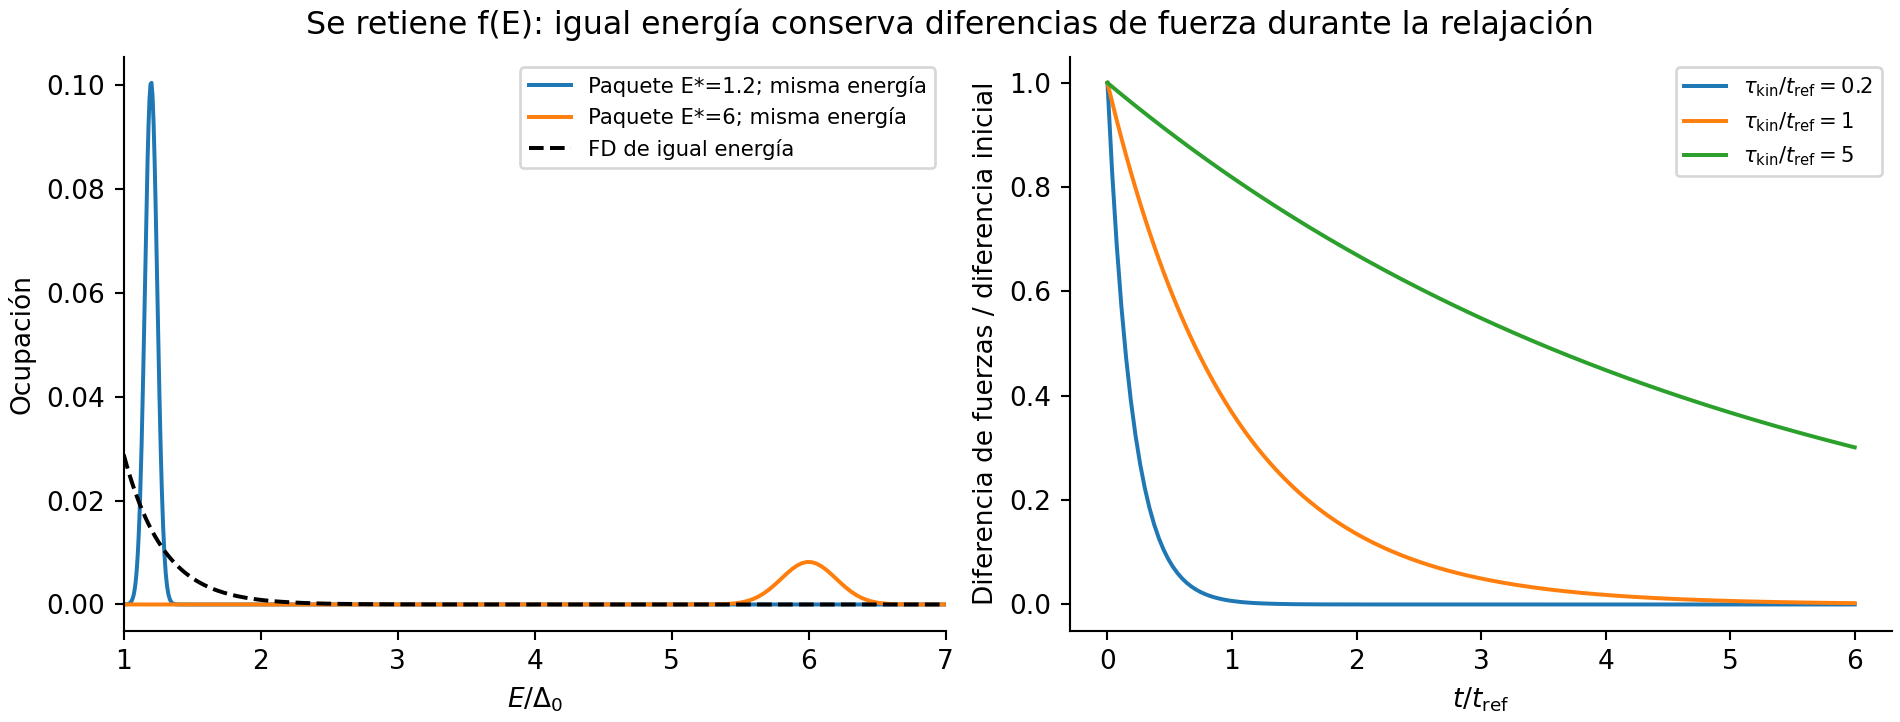
\includegraphics[width=0.98\linewidth,height=\textheight,keepaspectratio,alt={Figura B.2. Prueba nueva de poblaciones BCS a espectro fijo. Izquierda: dos paquetes de igual energía y su FD equivalente. Derecha: la diferencia de fuerzas entre ambos decae según el tiempo de relajación elegido; se conserva la energía durante toda la trayectoria. Ningún eje temporal está calibrado a NbN.}]{../figuras/B_07_espectro_y_relajacion.png}
\caption{Figura B.2. Prueba nueva de poblaciones BCS a espectro fijo.
Izquierda: dos paquetes de igual energía y su FD equivalente. Derecha:
la diferencia de fuerzas entre ambos decae según el tiempo de relajación
elegido; se conserva la energía durante toda la trayectoria. Ningún eje
temporal está calibrado a NbN.}
\end{figure}

Se usan paquetes gaussianos centrados en \(E/\Delta_0=1.2\) y \(6\), con
anchuras \(0.045\) y \(0.2\). Se conserva el estado de prueba de 0.3:
\(u_{\rm qp}/(4N_0\Delta_0^2)=0.025\) y \(k_BT_E/\Delta_0=0.2844346\).
El script fija \(N_0=\Delta_0=1\) y, por ello, integra una energía total
\(u_{\rm qp}=0.1\). El cociente de fuerzas es \(25.1873\). La
comparación con una integración adaptativa independiente coincide a
\(7.55\times10^{-15}\) relativo; la energía durante las trayectorias de
relajación cambia menos de \(2.78\times10^{-16}\) absoluto. El cociente
repite la comprobación necesaria de 0.3 con cuadraturas nuevas; la
evolución y la sensibilidad a \(\tau_{\rm kin}\) son pruebas de 0.4.

La diferencia de fuerzas caracteriza las poblaciones y no predice un
factor 25 de cambio en la latencia.

\section{B.6. Identidades térmicas para verificar el operador
espectral}\label{b.6.-identidades-tuxe9rmicas-para-verificar-el-operador-espectral}

\textbf{Propósito.} Conservar límites exactos con los que comprobar el
modelo elegido. Esta sección no define un segundo régimen de evolución
ni un cambio de representación: se insertan poblaciones FD como estados
de prueba del operador espectral.

Para electrones Fermi--Dirac, las identidades de balance detallado son

\[
\mathcal B_S=[f(E)-f(E+\Omega)]
[n_B(\Omega,T_e)-n(\Omega)], \tag{B.24}
\]

\[
\mathcal B_R=[1-f(E)-f(\Omega-E)]
[n_B(\Omega,T_e)-n(\Omega)]. \tag{B.25}
\]

La segunda se obtiene usando
\((1-f_E)(1-f_{\Omega-E})=e^{\Omega/k_BT_e}f_Ef_{\Omega-E}\).

Para la primera,
\(f(E+\Omega)[1-f(E)]=e^{-\Omega/k_BT_e}f(E)[1-f(E+\Omega)]\). Con
\(n_B=(e^{\Omega/k_BT_e}-1)^{-1}\) se factoriza B.3 y aparece B.24.
Cuando \(n=n_B(T_e)\) ambos balances netos se anulan \textbf{para cada
par de energías}, antes de integrar. Esto es balance detallado; una
potencia integrada cero por cancelación entre canales sería una prueba
más débil. Se definen

\[
J_S(\Omega;T_e,|\Delta|,q)=\int_0^\infty
\mathcal C_S(E,E+\Omega)[f(E)-f(E+\Omega)]\,dE, \tag{B.26}
\]

\[
J_R(\Omega;T_e,|\Delta|,q)=\int_0^\Omega
\mathcal C_R(E,\Omega-E)[1-f(E)-f(\Omega-E)]\,dE. \tag{B.27}
\]

Entonces

\[
\begin{gathered}
\mathcal G_\Omega=\frac{4\pi N_0}{\hbar}\alpha^2F(\Omega)\Omega(2J_S+J_R),\\
P_{e\text{-ph}}=\int_0^\infty\mathcal G_\Omega
[n_B(\Omega,T_e)-n(\Omega)]\,d\Omega.
\end{gathered} \tag{B.28}
\]

La ecuación fonónica se convierte en

\[
\begin{gathered}
\dot n=\gamma_{\rm ph}(\Omega;T_e,|\Delta|,q)
[n_B(\Omega,T_e)-n]-\frac{n-n_b}{\tau_{\rm esc}},\\
\gamma_{\rm ph}=\frac{\mathcal G_\Omega}{g_{\rm ph}(\Omega)\Omega}.
\end{gathered} \tag{B.29}
\]

Se evalúa el cociente únicamente donde existen modos; fuera de ese
soporte no hay una variable fonónica física que deba dividirse por cero.
B.29 es un límite verificable del operador completo; el modelo 0.4 sigue
evaluando B.3--B.6 para la población real.

\subsection{B.6.1. Prueba del límite
normal}\label{b.6.1.-prueba-del-luxedmite-normal}

En el estado normal, \(\mathcal C_S=\mathcal C_R=1\):

\[
\begin{gathered}
J_S=\int_0^\Omega f(E)dE,\\
J_R=\Omega-2\int_0^\Omega f(E)dE.
\end{gathered}
\]

Por tanto,

\[
2J_S+J_R=\Omega. \tag{B.30}
\]

La potencia normal queda

\[
P_{e\text{-ph}}^{n}=\frac{4\pi N_0}{\hbar}
\int_0^\infty\alpha^2F(\Omega)\Omega^2
[n_B(\Omega,T_e)-n(\Omega)]\,d\Omega. \tag{B.31}
\]

Si adicionalmente \(\alpha^2F\propto\Omega^2\) en el intervalo relevante
y los fonones son térmicos, aparece una ley \(T_e^5-T_{\rm ph}^5\). No
debe imponerse esa ley a un espectro completo fuera del intervalo
acústico correspondiente.

La prueba nueva de trayectoria de B.10 comprueba el balance detallado
antes de excitar la burbuja: el máximo valor del operador en equilibrio
común es \(1.92\times10^{-18}\) en sus unidades. Las identidades
B.30--B.31 siguen siendo referencias analíticas. No se vuelven a
presentar las cifras de cuadratura térmica de 0.3 como mediciones
nuevas.

\subsection{B.6.2. Conductividad térmica del mismo
espectro}\label{b.6.2.-conductividad-tuxe9rmica-del-mismo-espectro}

Al insertar \(\nabla f=(\partial f/\partial T_e)\nabla T_e\) en B.14,

\[
\kappa_s(T_e,|\Delta|,q)=\frac{4N_0D}{k_BT_e^2}
\int_0^\infty E^2\mathcal D_L(E)
 f_{\rm FD}(1-f_{\rm FD})\,dE. \tag{B.32}
\]

Con \(\mathcal D_L=1\), se recupera
\(\kappa_n=(\pi^2k_B^2/3e^2)\sigma_nT_e\). Esta prueba verifica
simultáneamente unidades, espín y normalización. La expresión nueva
retiene la dependencia de depairing que no estaba presente en la
conductividad BCS \(\kappa_s(T_e,|\Delta|)\) de producción.

\section{B.7. Contrato continuo, bordes y admisión de
datos}\label{b.7.-contrato-continuo-bordes-y-admisiuxf3n-de-datos}

\subsection{B.7.1. Una sola ecuación electrónica en todo el
tiempo}\label{b.7.1.-una-sola-ecuaciuxf3n-electruxf3nica-en-todo-el-tiempo}

Las piezas anteriores forman la ecuación fuerte

\[
\begin{aligned}
4N_0\rho\left(\left.\partial_tf\right|_E
+\left.\dot E\right|_x\partial_Ef\right)
={}&-\nabla\cdot\boldsymbol\Phi_f+\mathcal J_{e\text{-ph}}\\
&+4N_0\rho\left[\frac{f_{\rm FD}(E,T_E)-f}{\tau_{\rm kin}}+\mathcal H(E)\right].
\end{aligned}
\tag{B.33}
\]

\(\mathcal H(E)\) es B.41 evaluada en el estado correspondiente. El
término de colisión electrónica queda especificado sin ambigüedad por
las mismas reacciones que actualizan los fonones:

\[
\begin{aligned}
\mathcal J_{e\text{-ph}}(\varepsilon)
={}&\int_0^\infty d\Omega\int_0^\infty dE\,
[\delta_D(\varepsilon-E)-\delta_D(\varepsilon-E-\Omega)]\mathcal R_S\\
&-\int_0^\infty d\Omega\int_0^\Omega dE\,
[\delta_D(\varepsilon-E)+\delta_D(\varepsilon-\Omega+E)]\mathcal R_R.
\end{aligned}
\tag{B.34}
\]

\(\delta_D\) es la delta de Dirac, que selecciona la energía de llegada
o salida; no es el parámetro de núcleo \(\delta\) de C. Multiplicar B.34
por cualquier peso e integrar reproduce B.7. Se evalúa B.33 sobre
estados existentes; en regiones de DOS nula no se divide por \(\rho\).
La coordenada \(p(x)\) de B.43 es la representación de evolución
adoptada. Para calcular difusión, se reconstruye el gradiente a
\textbf{la misma energía} en las celdas vecinas; igualar sus índices
\(x\) cuando tienen gaps distintos transportaría estados de energías
diferentes.

\subsection{B.7.2. Densidad de modos: unidad y normalización
explícitas}\label{b.7.2.-densidad-de-modos-unidad-y-normalizaciuxf3n-expluxedcitas}

Se adopta como entrada primaria \(g_{\rm ph}(\Omega)\), número de modos
por volumen y energía {[}J\(^{-1}\)m\(^{-3}\){]}. Si un archivo declara
una DOS \(F_\nu\) por átomo y por THz, la transformación es

\[
\Omega=h\,10^{12}\nu_{\rm THz},\qquad
g_{\rm ph}(\Omega)
=\frac{n_{\rm at}F_\nu(\nu_{\rm THz})}{h\,10^{12}}.
\tag{B.35}
\]

Aquí \(h=2\pi\hbar\) y \(n_{\rm at}\) es la densidad de átomos; el
escenario existente usa \(48\) nm\(^{-3}\). Para una DOS completa por
átomo, \(\int g_{\rm ph}d\Omega=3n_{\rm at}\). Si el proveedor entrega
una DOS por celda con \(s\) átomos, se convierte primero a la convención
por átomo dividiendo entre \(s\); no se multiplica esa DOS directamente
por una densidad de átomos. Una DOS parcial debe identificar qué modos
cuenta y su densidad; no satisface por obligación la integral de todos
los modos.

\textbf{Resultado de la auditoría 0.4.} El archivo
\nolinkurl{nbn-a2f-ph.dat} de Geminga tiene 11999 filas, eje 0--20 THz y
cabecera \nolinkurl{PhDOS\ (st/THz)}. Su integral es \(0.7084201\), no
\(3\) por átomo; el peso negativo integrado es \(-0.0115301\), un
\(1.60\%\) del positivo. Eliminarlo daría \(0.7199501\), lo que tampoco
resuelve la normalización.

\begin{figure}
\centering
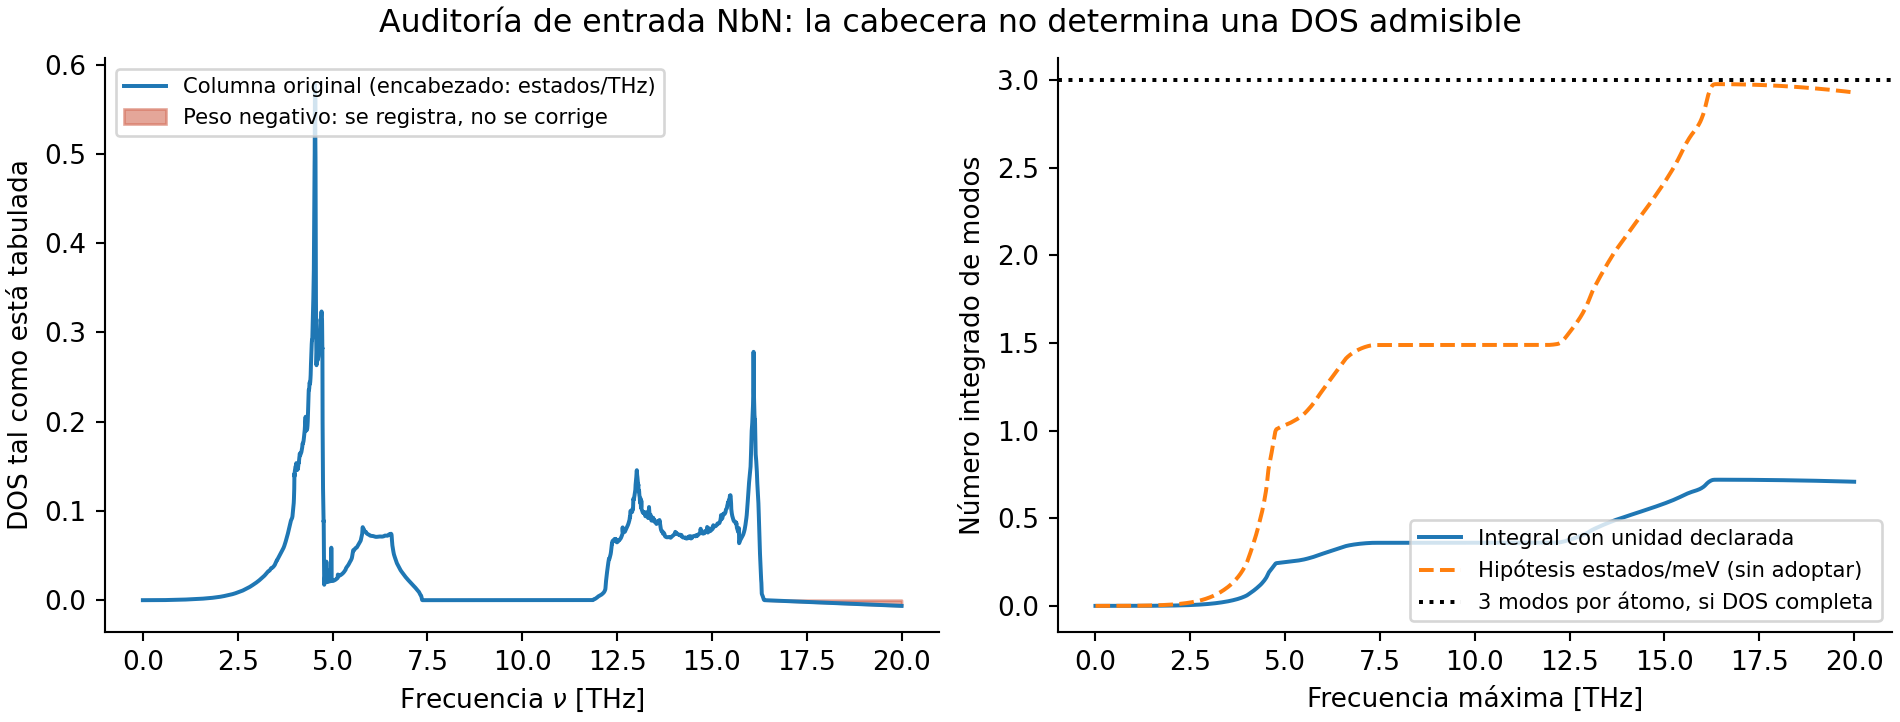
\includegraphics[width=0.98\linewidth,height=\textheight,keepaspectratio,alt={Figura B.3. Auditoría del archivo material suministrado, sin modificarlo. La integral no satisface la normalización declarada. La línea discontinua muestra una hipótesis de unidad que explica aproximadamente el factor, pero no se adopta como corrección.}]{../figuras/B_06_auditoria_dos.png}
\caption{Figura B.3. Auditoría del archivo material suministrado, sin
modificarlo. La integral no satisface la normalización declarada. La
línea discontinua muestra una hipótesis de unidad que explica
aproximadamente el factor, pero no se adopta como corrección.}
\end{figure}

Hay una pista verificable: si la columna fuera estados/meV, aunque la
cabecera diga estados/THz, el factor \(h=4.135667696\) meV/THz
produciría una integral bruta \(2.929790\) y positiva \(2.977475\),
cercana a tres. Es una inferencia sobre una posible discrepancia de
unidades, no una identificación de su origen. Se requiere documentación
del proveedor sobre unidad, normalización y cola negativa. \textbf{Esta
entrada queda inadmisible para energías y tasas fonónicas absolutas de
0.4 hasta resolverlo.} No se reescala ni se recorta automáticamente. El
valor \(\lambda=1.215665\) de la otra columna es sólo su integral; no
valida la DOS fonónica.

\subsection{B.7.3. Dominio y condiciones de
contorno}\label{b.7.3.-dominio-y-condiciones-de-contorno}

El dominio cinético es la película bidimensional \(\mathcal W\), con
espesor uniforme \(d\), desde el instante de transferencia \(t_0\) hasta
el final de la ventana de simulación. En contactos electrónicos ideales
con reservorios a \(T_b>0\) se fija Fermi--Dirac; los bordes laterales
son aislantes:

\[
f\big|_{\partial\mathcal W_{\rm contacto}}=f_{\rm FD}(E,T_b),
\qquad
\widehat{\mathbf n}\cdot\boldsymbol\Phi_f\big|_{\partial\mathcal W_{\rm lateral}}=0.
\tag{B.36}
\]

En una interfaz transparente entre sectores 2D y 1D del mismo material,
se acoplan \(f(E)\) y el flujo normal a igual energía, con las áreas
correspondientes en el balance. No se impone continuidad de \(p(x)\)
entre espectros diferentes. El remapeo entre \(E\) y \(x\) debe
conservar los conteos y la energía compartida en la interfaz. Los
fonones evolucionan localmente mediante B.10, sin derivadas espaciales,
por lo que no se añade una condición lateral ficticia; su reservorio es
\(n_b=n_B(\Omega,T_b)\) en el término de escape. Las fuentes ópticas
continuas son cero para \(t>t_0\): la energía del evento ya se depositó
en la condición inicial B.38--B.39. C y D fijan los bordes del
condensado y del circuito.

La admisión de una entrada espectral completa exige, además de unidades
trazables,

\[
\begin{gathered}
g_{\rm ph}\geq0,\quad \alpha^2F\geq0,\quad
\operatorname{supp}(\alpha^2F)\subseteq\operatorname{supp}(g_{\rm ph}),\\
\int_0^\infty g_{\rm ph}(\Omega)d\Omega=3n_{\rm at}.
\end{gathered}
\tag{B.37}
\]

La malla debe cubrir la energía retenida y los destinos de las
reacciones, con convergencia comprobada al ampliar corte y refinar. Un
canal fuera de la malla no es escape al sustrato: se amplía el soporte o
se rechaza la trayectoria. Se auditan \(0\leq f\leq1\), \(n\geq0\), la
inversión B.20 y los balances sin reparar poblaciones por recorte. La
prueba de B.10 comparte cada evento y cada flujo entre sus dos balances;
la convergencia del caso superconductivo con espectro móvil sigue siendo
una verificación de implementación pendiente, identificada en D.

\section{B.8. Condición inicial tras la
absorción}\label{b.8.-condiciuxf3n-inicial-tras-la-absorciuxf3n}

\textbf{Propósito.} Declarar qué energía y qué distribución entrega la
parte no resuelta de la cascada al intervalo que sí se modela. La
absorción óptica, el reparto entre excitaciones y la pérdida al sustrato
son pasos distintos.

Se condiciona el problema a que el fotón haya sido absorbido en la
película. Su probabilidad de absorción pertenece al problema óptico.
Después de esa absorción, las ramificaciones de la cascada distribuyen
la energía entre electrones y fonones; parte puede abandonar la
película. Las fluctuaciones de Fano describen variaciones estadísticas
de ese reparto. El factor de Fano caracteriza una varianza, no la
probabilidad de absorción ni la eficiencia cuántica del detector {[}K,
§§I--II{]}.

Sea \(t_0\) el instante en que comienza la descripción resuelta,
\(E_{\rm in}\) la energía excedente que recibe y \(u_\gamma(\mathbf r)\)
su densidad inicial. La normalización B.38 se explicita en esta versión
como

\[
\begin{gathered}
\int_{\mathcal V}u_\gamma(\mathbf r)\,dV=E_{\rm in},\\
E_{\rm in}=E_\gamma-E_{\rm perdido}^{<t_0}.
\end{gathered} \tag{B.38}
\]

Aquí se cuenta únicamente la energía del fotón; el trabajo posterior de
la fuente eléctrica entra en B.40. Si se empieza antes de toda pérdida,
\(E_{\rm in}=E_\gamma\). Si se empieza después de una etapa que ya
perdió energía, no corresponde depositar nuevamente el fotón completo.
En particular, una realización que retiene menos energía no representa
``una fracción de fotón absorbido'': representa un fotón absorbido cuya
energía fue repartida entre la película y su entorno.

Allmaras et al.~modelan la energía disponible al terminar la cascada
como una variable fluctuante y relacionan esa variación con latencia y
jitter {[}A19, §II, pp.~2--4 del preprint{]}. Una parametrización
efectiva de ese ensamble es

\[
\langle E_{\rm in}\rangle=\chi E_\gamma,
\qquad
\operatorname{Var}(E_{\rm in})\simeq F_{\rm eff}\,\varepsilon E_\gamma.
\tag{B.38a}
\]

\(\chi\) es la fracción media retenida; \(F_{\rm eff}\) es adimensional
y \(\varepsilon\) fija su convención energética. En la convención de
{[}K{]}, \(2\varepsilon\) es la energía media necesaria para generar un
par de QP. Conocer la media no determina la varianza. La definición
usual para un número de excitaciones es
\(F_N=\operatorname{Var}(N)/\langle N\rangle\); trasladarla a B.38a
exige especificar qué sectores y pérdidas representa la energía efectiva
{[}K, pp.~054507-4--5; A19, ecuación (6) del preprint{]}.

Si se conserva toda la energía del fotón en electrones \textbf{más}
fonones, \(E_{\rm in}=E_\gamma\) en cada evento y su varianza total es
cero. Aun así pueden fluctuar el número de QP y el reparto entre
sectores. Por ello no se puede asignar automáticamente la varianza Fano
de QP a la energía total de B.38: para esa energía,
\(F_{\rm eff}\varepsilon\) sólo debe resumir pérdidas fluctuantes o
sectores que quedaron fuera de la descripción. Cuando se modelan
explícitamente reparto y escape, esas fluctuaciones se generan allí y no
se añaden nuevamente mediante B.38a.

Como ejemplo mínimo, la tesis considera \(N\) fonones de igual energía
\(\bar\Omega\), cada uno retenido independientemente con probabilidad
\(r\). Si toda la energía inicial está en ellos,
\(N\bar\Omega=E_\gamma\), y el número retenido es binomial. Por ello

\[
\langle E_{\rm in}\rangle=rE_\gamma,
\qquad
\operatorname{Var}(E_{\rm in})
=\bar\Omega E_\gamma r(1-r).
\tag{B.38b}
\]

Es una derivación de la dispersión por escape, bajo esas hipótesis, y no
la cascada completa {[}A, §2.4.4, ecuación (2.51), pp.~44--46{]}. En el
modelo general los fonones tienen distintas energías, trayectorias y
probabilidades de transmisión. Se debe respetar
\(0\leq E_{\rm in}\leq E_\gamma\); una aproximación gaussiana estrecha
como la de {[}A19, ecuación (2){]} no autoriza colas de energía
imposibles. Una implementación que trunque esa distribución debe
normalizarla y comprobar los momentos efectivamente obtenidos.

\begin{figure}
\centering
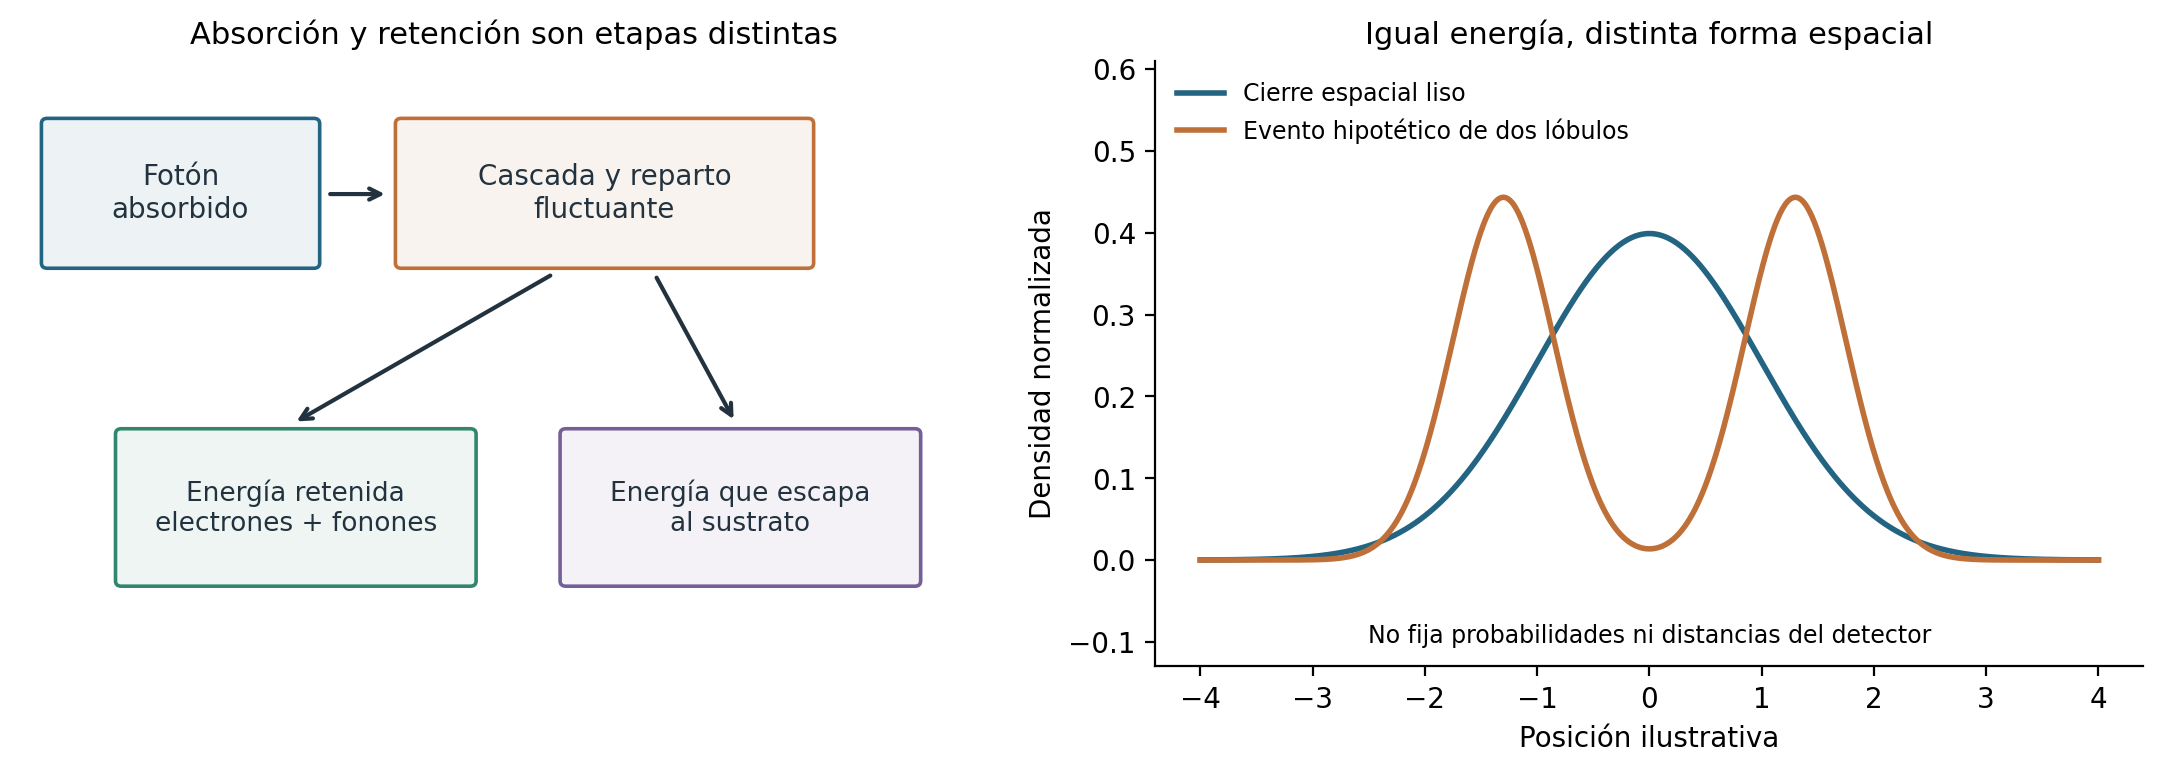
\includegraphics[width=0.98\linewidth,height=\textheight,keepaspectratio,alt={Figura B.4. Esquema pedagógico: tras una absorción, la cascada redistribuye la energía y puede perder parte al sustrato. Un perfil medio compacto no fija la forma de cada evento. Los dos lóbulos del ejemplo representan una posibilidad de una descripción espacial estocástica, no una predicción de frecuencia ni de separación.}]{../figuras/B_05_burbuja_y_retencion.png}
\caption{Figura B.4. Esquema pedagógico: tras una absorción, la cascada
redistribuye la energía y puede perder parte al sustrato. Un perfil
medio compacto no fija la forma de cada evento. Los dos lóbulos del
ejemplo representan una posibilidad de una descripción espacial
estocástica, no una predicción de frecuencia ni de separación.}
\end{figure}

Se adopta la burbuja fonónica posterior a la cascada de alta energía,
motivada por el peso de acoplamiento de {[}S, §III y apéndice{]}. Su
forma y normalización son

\[
\delta n(\Omega,\mathbf r,t_0)=
\frac{u_\gamma(\mathbf r)\,\alpha^2F(\Omega)}
{g_{\rm ph}(\Omega)\int_0^\infty\Omega\alpha^2F(\Omega)d\Omega}.
\tag{B.39}
\]

Multiplicar B.39 por \(g_{\rm ph}(\Omega)\Omega\) e integrar devuelve
exactamente \(u_\gamma\). Esa comprobación fija su energía, no su
validez espectral. El reparto inicial adoptado asigna B.38 a los
fonones; no se añade además un salto electrónico o una segunda
deposición fotónica. El condensado puede iniciarse continuo y
evolucionar mediante su fuerza no térmica, sin un salto impuesto a su
mínimo de equilibrio.

\textbf{La localización es una hipótesis estadística, no una prohibición
de separarse.} Nada obliga a las excitaciones iniciales a seguir juntas.
La dispersión elástica repetida borra su dirección inicial en el régimen
difusivo; una escala de expansión en dos dimensiones es \(\sqrt{4Dt}\),
no una distancia máxima permitida. Antes de alcanzar ese régimen deben
compararse vuelos \(v\tau\) y libres recorridos con el tamaño de la
región; los fonones pueden requerir transporte balístico aunque los
electrones sean difusivos. Una realización puede producir dos
concentraciones separadas si las ramas transportan suficiente energía
antes de dispersarla. Que además formen dos hotspots que supriman el
condensado depende de su separación, energía y posterior difusión. Ésta
es una inferencia física sobre trayectorias que el cierre de promedio no
resuelve: los cálculos radiales de {[}A, §2.3.2{]} apoyan una población
media localizada en sus condiciones, pero no calculan la probabilidad de
esos eventos. Cuantificarla requiere cascadas espaciales estocásticas;
una gaussiana central no puede descartarla por construcción.

En 0.4 se adopta una condición inicial determinista después de la
cascada omitida: \(f(t_0)=f_{\rm FD}(T_b)\), condensado continuo y toda
la energía retenida en la burbuja fonónica B.39. \(E_{\rm in}\),
\(t_0\), el centro y la anchura son datos de transferencia; no se
muestrean fluctuaciones Fano ni bifurcaciones espaciales en el candidato
de esta revisión. Se usa un perfil gaussiano normalizado sobre la
película: \(u_\gamma=E_{\rm in}w(\mathbf r)/d\),
\(\int_{\mathcal W}w\,d^2r=1\); la anchura nominal heredada es \(10\)
nm, sin atribuirle una medición nueva. Si se resuelve el escape
posterior mediante B.12, no se aplica además una fracción que incluya
esa misma pérdida. La energía sólo cambia por canales identificados,
aunque la población sea aleatoria. Como \(E_{\rm in}\) ya designa
energía retenida dentro de la película, normalizar \(w\) sobre ese
dominio conserva su significado. Para eventos próximos al borde, el
perfil y la energía transferidos deben corresponder a ese confinamiento;
normalizar una gaussiana no calcula las pérdidas previas. El tiempo
desde \(t_0\) debe distinguirse de la latencia desde el instante óptico
absoluto.

\section{B.9. Energía del condensado y fuentes de
calentamiento}\label{b.9.-energuxeda-del-condensado-y-fuentes-de-calentamiento}

\textbf{Propósito.} Evitar que recuperar amplitud cree o destruya
energía en el balance total. La energía del estado de fondo y la de las
excitaciones son partes distintas de la misma contabilidad electrónica.

El balance de una celda no se cierra sumando a la ecuación antigua dos
derivadas de almacenamiento y conservando sin cambios todas las fuentes.
La potencia reversible de superflujo, la disipación del parámetro de
orden y el trabajo eléctrico deben contarse una vez. C deriva la
identidad completa.

Para electrones térmicos, la forma resultante es

\[
\begin{aligned}
C_e\dot T_e={}&\nabla\cdot(\kappa_s\nabla T_e)
+\sigma_nE^2+Q_\Delta\\
&-P_{e\text{-ph}}+S_{\gamma,e}^{(E)}\\
&+T_e f_{T|\Delta|}\partial_t|\Delta|+T_e\partial_T\partial_{\mathbf q}f\cdot\dot{\mathbf q}.
\end{aligned}
\tag{B.40}
\]

\(f=f_e^{\rm FD}\) y \(Q_\Delta\geq0\) es la disipación del condensado.

\(S_{\gamma,e}^{(E)}\) representa una fuente electrónica resuelta; vale
cero si la absorción ya quedó incorporada como condición inicial. Los
subíndices de \(f\) indican derivadas parciales:
\(f_{T|\Delta|}=\partial_T\partial_{|\Delta|}f\). Es una ecuación
invertible y consistente con el funcional, no un uso ad hoc de
\(j_s\cdot E\) como calentamiento siempre positivo.

En todo el cálculo espectral,
\(P_{\rm heat}=\sigma_n|\mathbf E|^2+Q_\Delta\geq0\) se entrega a las
ocupaciones una sola vez. Se adopta el \textbf{cierre fenomenológico de
deposición espectral 0.4}:

\[
\begin{gathered}
T_*=\max(T_E,T_b)>0,\qquad f_*(E)=f_{\rm FD}(E,T_*),\\
\mathcal H(x)=\left.\dot p\right|_{\rm heat}
=\frac{P_{\rm heat}\,E(x)f_*(E(x))[1-p(x)]}
{4N_0\int_0^\infty E^2 f_*(E)[1-p]dx}.
\end{gathered}
\tag{B.41}
\]

El factor FD fija el reparto de la energía inyectada; la distribución
que evoluciona sigue siendo \(p(x)\). No se proyecta esa distribución a
FD. El denominador normaliza \(4N_0\int E\mathcal Hdx=P_{\rm heat}\). A
espectro fijo, \(\mathcal H\geq0\) si \(0\leq p\leq1\) y se anula en un
estado lleno, de modo que el campo continuo apunta hacia el intervalo de
Pauli. Con \(p=0\), \(T_*=T_b\) mantiene una fuente finita: no hace
falta sembrar ocupaciones arbitrarias.

Si \(p=f_{\rm FD}(T_E)\) y \(T_E\geq T_b\), B.41 reproduce exactamente
la dirección térmica \(E p(1-p)\) con la normalización energética
correspondiente. Los factores exponenciales se evalúan reescalados en
logaritmos cuando \(|\Delta|/(k_BT_*)\) es grande; ese reescalado común
cancela entre numerador y denominador. Una malla sin capacidad
electrónica disponible no admite una potencia positiva y debe ampliarse
o rechazar el estado, sin recortar energía.

\textbf{Diagnóstico que cambia 0.3.} La fuente anterior usaba
\(E p(1-p)\) también fuera de equilibrio. En el vacío su normalización
era cero; con dos semillas reducidas por \(10^{-12}\), daba fuerzas por
unidad de potencia \(0.6901\) y \(0.06209\) aunque ambas tendían a
población nula. La nueva fuente da \(0.9176\) en ambos límites, en las
unidades BCS de la prueba. Se reemplaza por B.41. La figura B.5 verifica
energía, límite térmico y una trayectoria desde \(p=0\). Esa corrección
determina un operador efectivo bien definido, pero \textbf{no deduce el
calentamiento microscópico de Keldysh}. Una integral de potencia no
puede fijar por sí sola cómo el campo o la relajación del condensado
crean excitaciones. La predicción de la forma espectral durante fuerte
disipación debe compararse con cinética impulsada o datos espectrales.
Tampoco se afirma producción de entropía positiva para toda población
invertida.

\begin{figure}
\centering
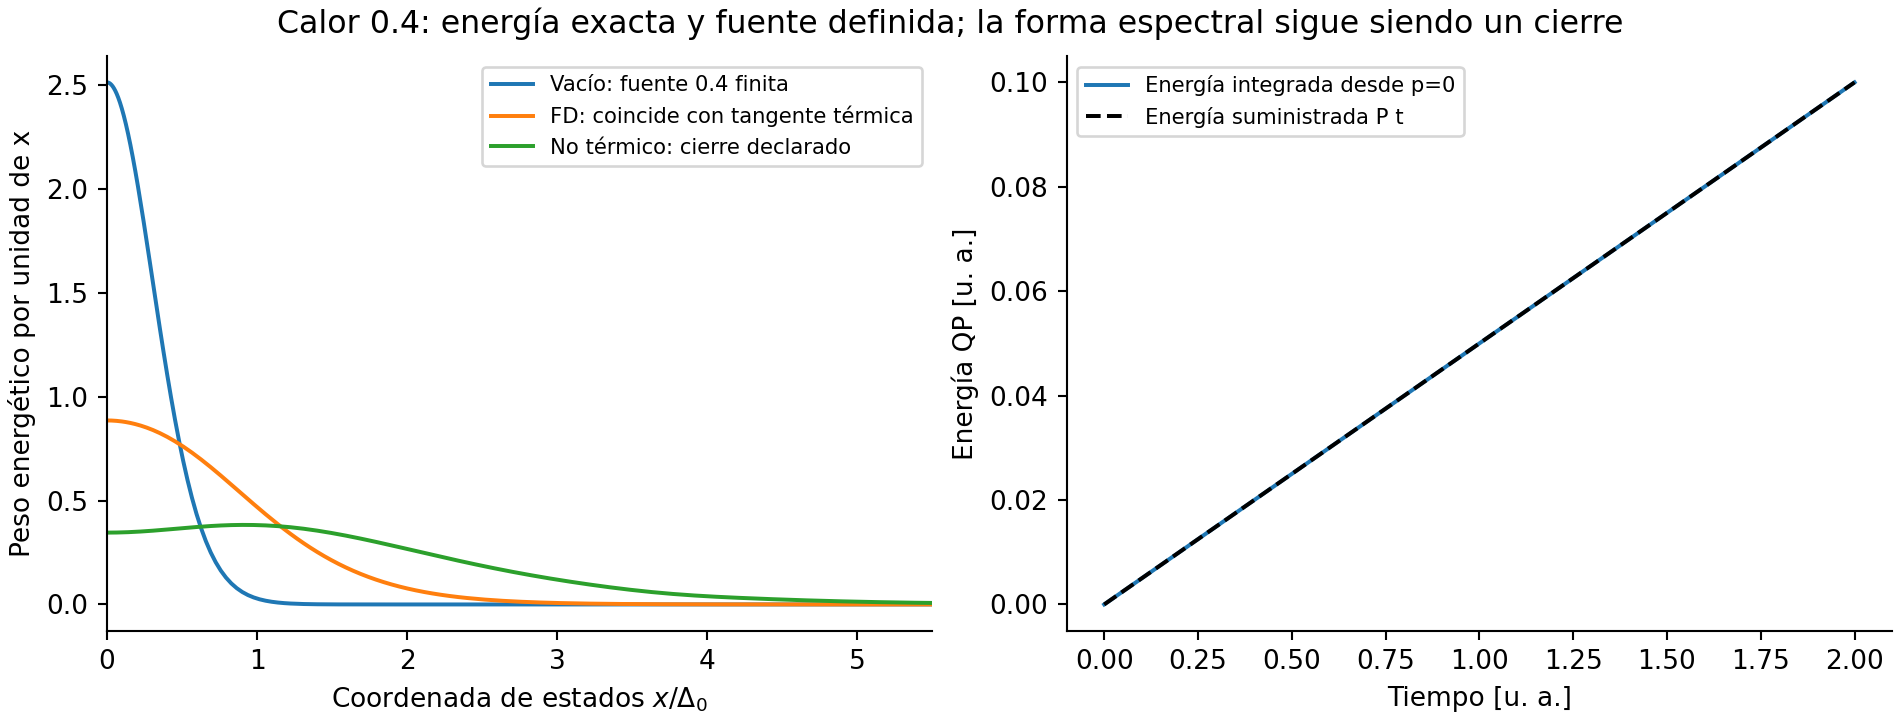
\includegraphics[width=0.98\linewidth,height=\textheight,keepaspectratio,alt={Figura B.5. Fuente de calor adoptada. Izquierda: reparto energético para vacío, FD y un paquete no térmico; cada curva está normalizada a la misma potencia. Derecha: energía integrada desde ocupación nula frente al trabajo suministrado. Es una prueba del cierre declarado, sin parámetros absolutos NbN.}]{../figuras/B_08_calor_espectral.png}
\caption{Figura B.5. Fuente de calor adoptada. Izquierda: reparto
energético para vacío, FD y un paquete no térmico; cada curva está
normalizada a la misma potencia. Derecha: energía integrada desde
ocupación nula frente al trabajo suministrado. Es una prueba del cierre
declarado, sin parámetros absolutos NbN.}
\end{figure}

La trayectoria usa \(E(x)=\sqrt{1+x^2}\), \(k_BT_b/\Delta_0=0.08\),
\(P=0.05\) y \(0\leq t\leq2\), en unidades declaradas del script.
Conserva \(u_{\rm qp}(t)=Pt\) a \(4.17\times10^{-17}\) absoluto y
mantiene \(0\leq p\leq0.028868\). Al pasar de 192 a 384 nodos, la fuerza
final cambia \(4.78\times10^{-11}\) relativo. El límite térmico de la
fuente coincide a \(5.26\times10^{-17}\) en norma integrada; estas
precisiones no son estimaciones del error físico del cierre.

\subsection{B.9.1. Celda aislada como prueba de
almacenamiento}\label{b.9.1.-celda-aislada-como-prueba-de-almacenamiento}

Para una celda homogénea sin corriente, fuentes, escape ni intercambio
fonónico, C da \(\partial_t|\Delta|=-\mathcal M X_{|\Delta|}\) y
\(Q_\Delta=\mathcal M X_{|\Delta|}^2\). Aquí
\(\mathcal M=1/\Gamma_{|\Delta|}>0\) es la movilidad, inversa de la
fricción de C. De \(u_e=f-Tf_T\) se obtiene, a \(q=0\),

\[
\dot u_e=(X_{|\Delta|}-T f_{T|\Delta|})\partial_t|\Delta|
+C_e\dot T.
\tag{B.42}
\]

Al sustituir B.40 se cancelan los términos mixtos y queda
\(\dot u_e=X_{|\Delta|}\partial_t|\Delta|+Q_\Delta=0\). Esta cancelación
explica el calentamiento durante la recuperación sin convertir todo el
cambio de amplitud en una fuente térmica adicional.

La identidad se mantiene como condición analítica de almacenamiento. Las
pruebas nuevas de C verifican el candidato integrado y su regularización
finita. B.10 añade la evolución de las poblaciones y del escape con sus
balances; ninguna de esas comprobaciones sustituye una comparación con
un transiente completo material.

\section{B.10. Verificaciones 0.4 y decisión de
admisión}\label{b.10.-verificaciones-0.4-y-decisiuxf3n-de-admisiuxf3n}

Se ejecutó \nolinkurl{sandbox/model_v0_4/checks_b_v04.py} en Geminga
con un hilo, Python 3.10.20, NumPy 2.2.6, SciPy 1.15.3 y Matplotlib
3.10.8. El programa es independiente del solver de producción y de los
scripts 0.3. Repite con cuadraturas independientes la prueba de paquetes
que justifica retener el espectro, y añade trayectorias de relajación,
calor y colisiones con transporte y escape.

{\def\LTcaptype{none} % do not increment counter
\begin{longtable}[]{@{}
  >{\raggedright\arraybackslash}p{(\linewidth - 4\tabcolsep) * \real{0.3333}}
  >{\raggedright\arraybackslash}p{(\linewidth - 4\tabcolsep) * \real{0.3333}}
  >{\raggedright\arraybackslash}p{(\linewidth - 4\tabcolsep) * \real{0.3333}}@{}}
\toprule\noalign{}
\begin{minipage}[b]{\linewidth}\raggedright
Prueba 0.4
\end{minipage} & \begin{minipage}[b]{\linewidth}\raggedright
Resultado
\end{minipage} & \begin{minipage}[b]{\linewidth}\raggedright
Qué permite concluir
\end{minipage} \\
\midrule\noalign{}
\endhead
\bottomrule\noalign{}
\endlastfoot
Paquetes BCS de igual energía & Cociente de fuerzas \(25.1873\);
cuadratura independiente \(7.55\times10^{-15}\) relativo & La energía
sola no conserva la fuerza \\
Relajación conservativa & Error energético \(2.78\times10^{-16}\);
sensibilidad a tres \(\tau_{\rm kin}\) & El cierre preserva energía y
Pauli; falta fijar su tiempo material \\
Calor desde el vacío & Error energético \(4.17\times10^{-17}\) & La
fuente nueva está definida y contabiliza la potencia \\
Refinamiento del calor, 192 a 384 nodos & Fuerza final cambia
\(4.78\times10^{-11}\) relativo & Estabilidad numérica de la prueba de
celda \\
Reacciones, difusión y escape & Residuo total \(2.02\times10^{-16}\)
relativo & La trayectoria de dos celdas intercambia energía de forma
consistente \\
Refinamiento de esa trayectoria, 24 a 48 intervalos electrónicos &
Energía QP final \(8.14\times10^{-5}\); escape \(1.04\times10^{-4}\)
relativo & Convergencia observada en el espectro normal sintético \\
Equilibrio común & Operador máximo \(1.92\times10^{-18}\) & Balance
detallado, además de conservación integrada \\
Archivo DOS NbN & Integral \(0.70842\) y peso negativo \(1.60\%\) del
positivo & No admitido para predicciones fonónicas absolutas \\
\end{longtable}
}

\begin{figure}
\centering
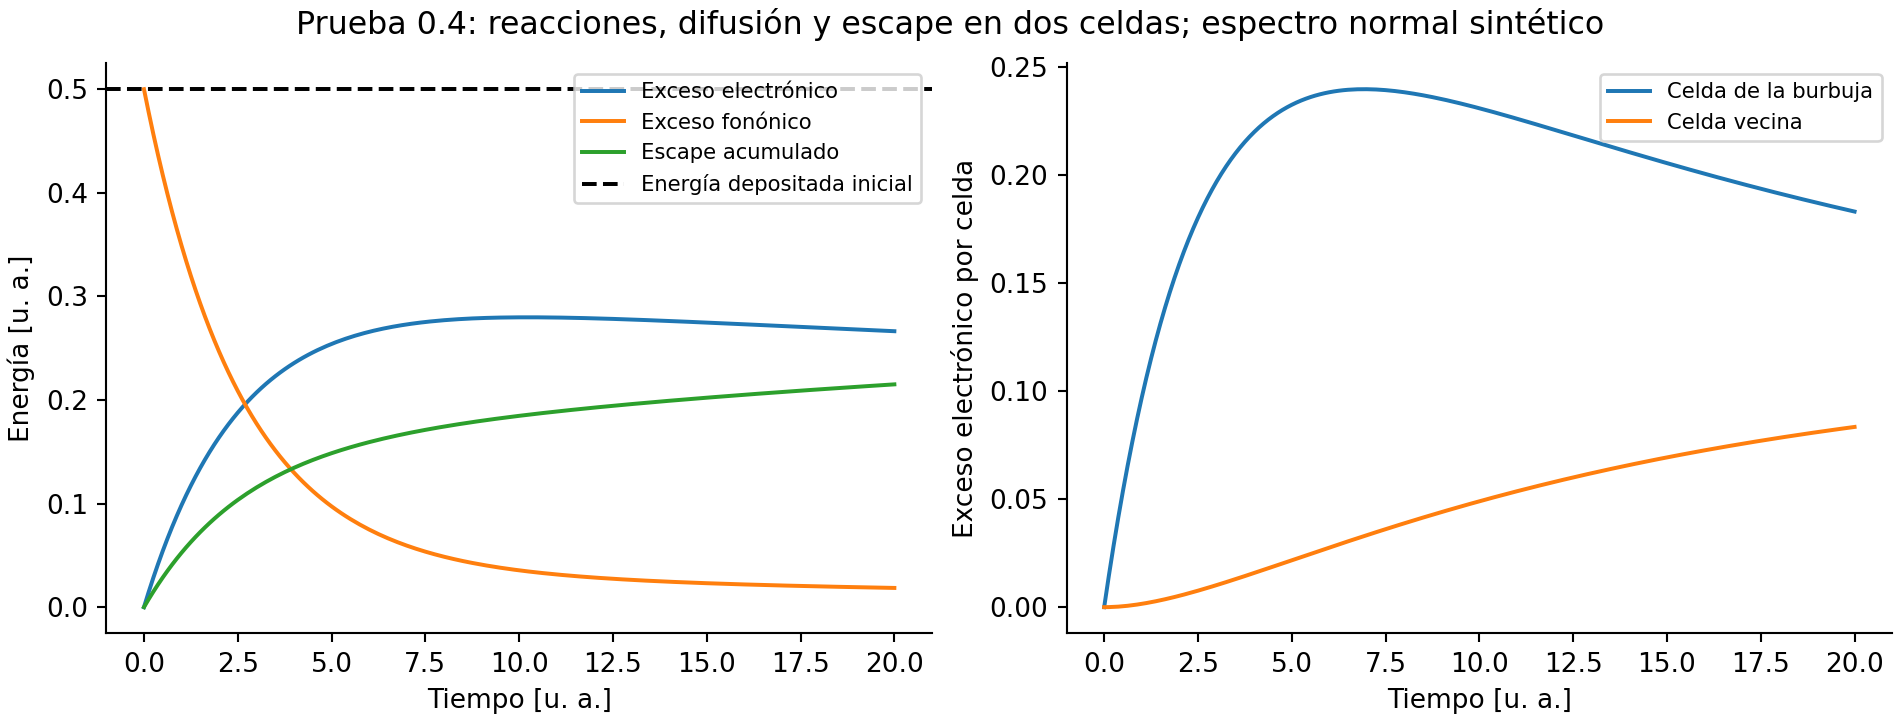
\includegraphics[width=0.98\linewidth,height=\textheight,keepaspectratio,alt={Figura B.6. Nueva trayectoria de dos celdas: la burbuja se deposita en la primera y las excitaciones electrónicas difunden a la segunda. La energía que sale por escape se registra por separado; al sumarla con ambas poblaciones se conserva la energía inicial. Ejes en unidades de un espectro normal sintético.}]{../figuras/B_09_trayectoria_conservativa.png}
\caption{Figura B.6. Nueva trayectoria de dos celdas: la burbuja se
deposita en la primera y las excitaciones electrónicas difunden a la
segunda. La energía que sale por escape se registra por separado; al
sumarla con ambas poblaciones se conserva la energía inicial. Ejes en
unidades de un espectro normal sintético.}
\end{figure}

La prueba utiliza DOS electrónica normal \(\rho=1\), espectro acústico
analítico \(\alpha^2F=0.03(\Omega/12)^2\), DOS Debye con densidad de
átomos 10 y corte \(\Omega_D=12\), difusión \(D=0.03\), escape
\(\tau_{\rm esc}=8\) y energía inicial adicional \(0.5\). Todas esas
cantidades están en unidades internas; no son un ajuste a NbN. Las
mallas tienen 12, 24 y 48 intervalos electrónicos, y el doble de
intervalos fonónicos. Cada reacción conecta energías cuya suma o
diferencia coincide exactamente; el mismo flujo cruza ambas celdas con
signos opuestos. Se integran \(0\leq t\leq20\) con tolerancias relativas
\(2\times10^{-9}\) y absolutas \(10^{-12}\). Las poblaciones se
mantienen físicas; no se aplican recortes. Sin escape, la prueba
separada conserva la energía con residuo relativo
\(4.01\times10^{-16}\).

\textbf{Admisión.} Queda cerrado el candidato matemático de B.33, B.10,
B.17 y B.41 con el espectro de C. Su uso para tiempos absolutos exige
una entrada fonónica admisible y un \(\tau_{\rm kin}\) identificado. La
implementación futura debe además verificar transporte entre espectros
diferentes, conservación al mover el gap, convergencia en
corte/energía/espacio/tiempo y sensibilidad del núcleo regularizado y de
la fuente de calor. Se registran como requisitos de comprobación del
candidato elegido, no como un menú de modelos pendiente de seleccionar.

Resultados reproducibles:
\nolinkurl{docs/modelo_v0_4/verificaciones/B_verificaciones_v04.json},
cuatro tablas CSV con prefijo \nolinkurl{B_04_} y figuras B\_06--B\_09.
El JSON incluye versiones de bibliotecas, hash del script, hash de la
entrada, tamaños de malla y residuos. Las ilustraciones de reacciones y
burbuja se conservan por su función pedagógica; no se vuelven a
etiquetar resultados antiguos como simulaciones nuevas.

\section{B.11. Energía adiabática y fuerzas de las
ocupaciones}\label{b.11.-energuxeda-adiabuxe1tica-y-fuerzas-de-las-ocupaciones}

\textbf{Propósito.} Derivar la energía interna y las fuerzas que utiliza
la cinética de B, a partir del espectro estático de A. Este desarrollo,
trasladado a B en 0.3, mantiene en A la construcción del catálogo
estático. C toma B.49--B.51 como derivadas locales de entrada y varía su
energía regularizada completa; no se deduce aquí la fricción del
condensado.

\subsection{B.11.1. Aproximación adiabática
adoptada}\label{b.11.1.-aproximaciuxf3n-adiabuxe1tica-adoptada}

La cinética quasiclásica y el término de desequilibrio de Vodolazov
proporcionan puntos de partida para acoplar una distribución no térmica
al condensado {[}V, S{]}. No basta con insertar un escalar de supresión
en cualquier ecuación dinámica y atribuirle toda esa teoría.

Se adopta una descripción \textbf{espectralmente adiabática,
electrón--hueco simétrica y localmente uniforme} después de la
excitación óptica no resuelta. El espectro responde instantáneamente a
\(|\Delta|\) y \(q\) dentro de esta aproximación; las ocupaciones pueden
seguir fuera de equilibrio. Su régimen de uso requiere comparar las
escalas temporales y espaciales. Las identidades que siguen corresponden
al espectro ideal causal, sin autoenergías adicionales que dependan de
la población. Un ensanchamiento fenomenológico arbitrario no viene
acompañado automáticamente de la misma termodinámica.

\subsection{B.11.2. Seguir estados cuando cambia su
energía}\label{b.11.2.-seguir-estados-cuando-cambia-su-energuxeda}

Si cambia el gap, los niveles se desplazan. Mantener fija una población
\textbf{de estados} no es lo mismo que mantener fija una función
tabulada en los mismos valores de energía. Para distinguirlo, definimos
la coordenada acumulada

\[
x(E;|\Delta|,\Gamma)=\int_0^E\rho(E';|\Delta|,\Gamma)\,dE',
\quad E=E(x;|\Delta|,\Gamma),\quad p(x)=f(E(x)).
\tag{B.43}
\]

\(x\) tiene unidades de energía y \(4N_0dx\) cuenta estados de
excitación positivos con el espín y la simetría electrón--hueco
adoptados. Es como numerar asientos en vez de nombrarlos por su altura:
al mover la estructura, la ocupación de cada asiento puede seguir siendo
la misma aunque cambie su energía. En BCS sin corriente,
\(x=\sqrt{E^2-|\Delta|^2}\) sobre el continuo. La inversa se define
sobre el soporte con estados; el intervalo vacío del gap no introduce
población.

Las derivadas de A.23 y de \((c^R)^2+(s^R)^2=1\) permiten relacionar el
movimiento de niveles con el espectro anómalo:

\[
\partial_{|\Delta|}\rho=-\partial_E R_2,
\qquad \partial_\Gamma\rho=\partial_E(N_2R_2).
\tag{B.44}
\]

Para explicitar el paso, al derivar \(|\Delta|c-\Gamma sc+izs=0\)
respecto del ángulo aparece

\[
K=-|\Delta|s-\Gamma(c^2-s^2)+izc,
\quad \partial_{|\Delta|}\Theta=-\frac{c}{K},
\quad \partial_E\Theta=-\frac{is}{K},
\quad \partial_\Gamma\Theta=\frac{sc}{K}.
\tag{B.44a}
\]

Por tanto \(\partial_{|\Delta|}c=i\partial_Es\) y
\(\partial_\Gamma c=-(i/2)\partial_E(s^2)\). Tomar partes reales da
B.44. Estas igualdades se entienden con el regulador causal y, si el
borde es singular, después de integrar antes de tomar \(\eta\to0^+\).

Para las ramas simétricas, \(R_2(0)=N_2(0)R_2(0)=0\). Integrando B.44 y
derivando B.43 a \(x\) fijo,

\[
\left.\frac{\partial E}{\partial|\Delta|}\right|_x=\frac{R_2}{\rho},
\qquad
\left.\frac{\partial E}{\partial\mathbf q}\right|_x
=-\hbar D\mathbf q\frac{N_2R_2}{\rho}.
\tag{B.45}
\]

Los cocientes se usan sobre el soporte espectral o mediante integrales;
no se divide puntualmente por la DOS dentro del gap.

\subsection{B.11.3. Energía y fuerzas de una población no
térmica}\label{b.11.3.-energuxeda-y-fuerzas-de-una-poblaciuxf3n-no-tuxe9rmica}

Sea \(U_{\rm vac}(|\Delta|,q)=\lim_{T\to0}f_e^{\rm FD}(T,|\Delta|,q)\),
manteniendo amplitud y superflujo fijos. La energía adiabática propuesta
es

\[
u_e[|\Delta|,\mathbf q;p]
=U_{\rm vac}(|\Delta|,q)
+4N_0\int_0^\infty E(x;|\Delta|,q)p(x)\,dx.
\tag{B.46}
\]

El primer término pertenece al fondo emparejado y al superflujo; el
segundo es la energía de sus excitaciones. A corriente nula,

\[
U_{\rm vac}(|\Delta|,0)
=N_0|\Delta|^2\left[\ln\frac{|\Delta|}{\Delta_0}-\frac12\right],
\qquad \Delta_0=\pi e^{-\gamma_E}k_BT_c.
\tag{B.47}
\]

\(\gamma_E\) es la constante de Euler. La entropía de ocupaciones es

\[
s_e[p]=-4k_BN_0\int_0^\infty
\{p\ln p+(1-p)\ln(1-p)\}\,dx.
\tag{B.48}
\]

Variando B.46 a \(p(x)\) fijo y utilizando B.45 junto con
\(dx=\rho\,dE\),

\[
\begin{aligned}
X_{|\Delta|}[p]
&=\left.\partial_{|\Delta|}u_e\right|_{p,q}\\
&=\partial_{|\Delta|}U_{\rm vac}
+4N_0\int_0^\infty R_2(E)f(E)\,dE,
\end{aligned}
\tag{B.49}
\]

\[
\boldsymbol\Pi[p]
=\left.\partial_{\mathbf q}u_e\right|_{p,|\Delta|}
=\frac{\hbar}{2e}\mathbf j_s[f].
\tag{B.50}
\]

La segunda identidad corresponde a la corriente del catálogo local y
utiliza también A.20 a \(T=0\): la población resta al valor de corriente
del vacío mediante el peso \(2N_2R_2\). En 0.4 se evalúa en
\(q=q_\delta\); la corriente física \(\mathbf j_\delta\) incluye además
la variación de ese argumento y del término de gradientes de C. Las dos
fuerzas son derivadas del \textbf{modelo adiabático B.46}; no
constituyen una demostración de un potencial termodinámico para todo
estado Keldysh, ni incluyen memoria temporal, desequilibrio de carga o
gradientes espectrales generales.

Minimizar \(u_e-Ts_e\) respecto de \(p(x)\) da \(E+k_BT\ln[p/(1-p)]=0\),
es decir, Fermi--Dirac. Sobre esa población, B.49 recupera A.19. Para la
temperatura equivalente de energía \(T_E\) definida en B.20, la
diferencia de fuerza es

\[
\delta X_{|\Delta|}
=4N_0\int_0^\infty R_2(E)
\left[f(E)-f_{\rm FD}(E,T_E)\right]\,dE.
\tag{B.51}
\]

Cerca de \(T_c\) se puede expresar esa fuerza como una corrección
escalar con la normalización GL apropiada. Fuera de ese régimen, B.51
mantiene explícitamente el peso energético y la escala de fuerza,
mientras el coeficiente disipativo sigue siendo un cierre por
contrastar.

\subsection{B.11.4. Igual energía no implica igual acción sobre el
condensado}\label{b.11.4.-igual-energuxeda-no-implica-igual-acciuxf3n-sobre-el-condensado}

Para un paquete estrecho sin corriente, centrado en \(E_*>|\Delta|\),

\[
\frac{\delta X_{|\Delta|}}{\delta u_{\rm qp}}
=\frac{R_2(E_*)}{E_*\rho(E_*)}
=\frac{|\Delta|}{E_*^2}.
\tag{B.52}
\]

Dos paquetes de igual energía en \(1.2|\Delta|\) y \(6|\Delta|\)
difieren en un factor \(25\) en esta aproximación de ancho despreciable.
El paquete de menor energía contiene más excitaciones, y cada una pesa
más en la fuerza de supresión. Ambos paquetes pueden tener la misma
\(T_E\) sin tener el mismo efecto sobre el condensado.

La figura B.2 muestra los paquetes de ancho finito, su comparación
térmica y la persistencia de su diferencia de fuerzas durante la
relajación; se conserva una sola copia en B.5.3.

Las cuadraturas nuevas de B.5.3 repiten este cociente y añaden su
relajación en tiempos reducidos. La coincidencia confirma la razón para
conservar el espectro, sin convertirla en una predicción de latencia.

\section{Referencias y procedencia}\label{referencias-y-procedencia}

{[}M{]} J. A. Díaz Monge, \nolinkurl{memoria_02.pdf}, 2026, anexo B,
pp.~impresas 113--120; anexo A.5 para la aproximación de coherencia.
Estado térmico de producción: \(P_\Delta\) y \(P_q\) omitidos y
deposición inicial en \(T_{\rm ph}\).

{[}V{]} D. Y. Vodolazov, \emph{Single-Photon Detection by a Dirty
Current-Carrying Superconducting Strip Based on the Kinetic-Equation
Approach}, Physical Review Applied \textbf{7}, 034014 (2017).
\href{https://doi.org/10.1103/PhysRevApplied.7.034014}{DOI};
\href{https://arxiv.org/pdf/1611.06060}{preprint}. Se cotejan las
ecuaciones (1)--(5), pp.~2--3, y §III, ecuaciones (16)--(22), pp.~4--6
del preprint: comparación de condiciones iniciales con igual energía. La
aproximación de volumen inicial fijo y escape despreciado corresponde a
esa prueba, no a una condición universal.

{[}S{]} A. Simon et al., \emph{Ab initio modeling of nonequilibrium
dynamics in superconducting detectors and qubits}, Physical Review B
\textbf{112}, 174512 (2025).
\href{https://doi.org/10.1103/3m2k-mzr6}{DOI};
\href{https://arxiv.org/html/2501.13791v3}{preprint v3 cotejado}. En v3,
ecuaciones (1a)--(1b), (6a)--(6e) y (8): colisiones y energía fonónica;
§VII.1, texto posterior a la ecuación (8): burbuja proporcional a
\(\alpha^2\) y su normalización; §II y figura 2: \(N\) como densidad de
iones y referencia Debye de tres modos por ion. No se atribuye a ese
artículo la unidad inconsistente de la copia DAT local. Las clases de E
sobre modos, DOS y DFPT conectan esas entradas con B.2--B.3.

{[}A{]} J. P. Allmaras, \emph{Modeling and Development of
Superconducting Nanowire Single-Photon Detectors}, tesis doctoral,
Caltech (2020). \href{https://thesis.caltech.edu/13748/}{Registro y
DOI};
\href{https://thesis.caltech.edu/13748/08/Allmaras_Thesis_Final.pdf}{PDF
oficial}. Copia cotejada de 259 páginas,
\nolinkurl{Allmaras_Thesis_Final.pdf}: §2.3.1, pp.~impresas 19--20 (PDF
31--32), primera generación de fonones; §2.3.2, pp.~20--24 (PDF 32--36),
difusión; §2.4.4, pp.~44--46 (PDF 56--58), ecuaciones (2.51)--(2.52),
fluctuaciones de escape; §2.4.6, pp.~50--53 (PDF 62--65), corrección
efectiva de la transferencia de la burbuja. Se verifica esta paginación
en 0.3.

{[}A19{]} J. P. Allmaras et al., \emph{Intrinsic Timing Jitter and
Latency in Superconducting Nanowire Single-photon Detectors}, Physical
Review Applied \textbf{11}, 034062 (2019).
\href{https://doi.org/10.1103/PhysRevApplied.11.034062}{DOI};
\href{https://arxiv.org/pdf/1805.00130v2}{preprint arXiv:1805.00130v2}.
Se coteja §II del preprint de 2018, pp.~2--4, ecuaciones (2), (5)--(7):
energía retenida fluctuante y efecto sobre latencia. La numeración
citada corresponde expresamente al preprint, no se presupone idéntica a
la edición publicada.

{[}K{]} A. G. Kozorezov et al., \emph{Fano fluctuations in
superconducting-nanowire single-photon detectors}, Physical Review B
\textbf{96}, 054507 (2017).
\href{https://doi.org/10.1103/PhysRevB.96.054507}{DOI};
\href{https://tsapps.nist.gov/publication/get_pdf.cfm?pub_id=920691}{PDF
publicado en NIST}. §§I--II, pp.~054507-1--5: ramificación entre
electrones y fonones, factor de Fano y escape; ecuaciones (11)--(12),
p.~054507-5, varianza efectiva. No se interpreta el factor de Fano como
eficiencia óptica.

{[}R{]} Repositorio \nolinkurl{pysnspd}:
\nolinkurl{configs/geminga_local_v3.yaml},
\nolinkurl{pysnspd/kinetic/eliashberg.py},
\nolinkurl{pysnspd/kinetic/power_table.py} y
\nolinkurl{pysnspd/excitation/photon.py}, inspeccionados como contexto de
entradas. El catálogo remoto auditado es
\nolinkurl{/home/jdiaz/scratch/big_data/catalogs/simon_2025/nbn-a2f-ph.dat},
hash SHA-256
\nolinkurl{e94f11273e6c42b7c8fad978b78d119166e241bec1614ee77e4176906fa8f5df}.
No se modifica el archivo ni el tratamiento de producción.

{[}Q{]} Verificaciones nuevas de 0.4:
\nolinkurl{sandbox/model_v0_4/checks_b_v04.py} y
\nolinkurl{docs/modelo_v0_4/verificaciones/B_verificaciones_v04.json},
con CSV y figuras de esta entrega. Ejecución independiente en Geminga,
un hilo. Los cálculos comprueban el candidato y sus requisitos de
entrada; no constituyen un transiente completo de SNSPD. D registra la
reproducción y sincronización.

\end{document}
